% Options for packages loaded elsewhere
\PassOptionsToPackage{unicode}{hyperref}
\PassOptionsToPackage{hyphens}{url}
%
\documentclass[
]{book}
\usepackage{amsmath,amssymb}
\usepackage{iftex}
\ifPDFTeX
  \usepackage[T1]{fontenc}
  \usepackage[utf8]{inputenc}
  \usepackage{textcomp} % provide euro and other symbols
\else % if luatex or xetex
  \usepackage{unicode-math} % this also loads fontspec
  \defaultfontfeatures{Scale=MatchLowercase}
  \defaultfontfeatures[\rmfamily]{Ligatures=TeX,Scale=1}
\fi
\usepackage{lmodern}
\ifPDFTeX\else
  % xetex/luatex font selection
\fi
% Use upquote if available, for straight quotes in verbatim environments
\IfFileExists{upquote.sty}{\usepackage{upquote}}{}
\IfFileExists{microtype.sty}{% use microtype if available
  \usepackage[]{microtype}
  \UseMicrotypeSet[protrusion]{basicmath} % disable protrusion for tt fonts
}{}
\makeatletter
\@ifundefined{KOMAClassName}{% if non-KOMA class
  \IfFileExists{parskip.sty}{%
    \usepackage{parskip}
  }{% else
    \setlength{\parindent}{0pt}
    \setlength{\parskip}{6pt plus 2pt minus 1pt}}
}{% if KOMA class
  \KOMAoptions{parskip=half}}
\makeatother
\usepackage{xcolor}
\usepackage{color}
\usepackage{fancyvrb}
\newcommand{\VerbBar}{|}
\newcommand{\VERB}{\Verb[commandchars=\\\{\}]}
\DefineVerbatimEnvironment{Highlighting}{Verbatim}{commandchars=\\\{\}}
% Add ',fontsize=\small' for more characters per line
\usepackage{framed}
\definecolor{shadecolor}{RGB}{248,248,248}
\newenvironment{Shaded}{\begin{snugshade}}{\end{snugshade}}
\newcommand{\AlertTok}[1]{\textcolor[rgb]{0.94,0.16,0.16}{#1}}
\newcommand{\AnnotationTok}[1]{\textcolor[rgb]{0.56,0.35,0.01}{\textbf{\textit{#1}}}}
\newcommand{\AttributeTok}[1]{\textcolor[rgb]{0.13,0.29,0.53}{#1}}
\newcommand{\BaseNTok}[1]{\textcolor[rgb]{0.00,0.00,0.81}{#1}}
\newcommand{\BuiltInTok}[1]{#1}
\newcommand{\CharTok}[1]{\textcolor[rgb]{0.31,0.60,0.02}{#1}}
\newcommand{\CommentTok}[1]{\textcolor[rgb]{0.56,0.35,0.01}{\textit{#1}}}
\newcommand{\CommentVarTok}[1]{\textcolor[rgb]{0.56,0.35,0.01}{\textbf{\textit{#1}}}}
\newcommand{\ConstantTok}[1]{\textcolor[rgb]{0.56,0.35,0.01}{#1}}
\newcommand{\ControlFlowTok}[1]{\textcolor[rgb]{0.13,0.29,0.53}{\textbf{#1}}}
\newcommand{\DataTypeTok}[1]{\textcolor[rgb]{0.13,0.29,0.53}{#1}}
\newcommand{\DecValTok}[1]{\textcolor[rgb]{0.00,0.00,0.81}{#1}}
\newcommand{\DocumentationTok}[1]{\textcolor[rgb]{0.56,0.35,0.01}{\textbf{\textit{#1}}}}
\newcommand{\ErrorTok}[1]{\textcolor[rgb]{0.64,0.00,0.00}{\textbf{#1}}}
\newcommand{\ExtensionTok}[1]{#1}
\newcommand{\FloatTok}[1]{\textcolor[rgb]{0.00,0.00,0.81}{#1}}
\newcommand{\FunctionTok}[1]{\textcolor[rgb]{0.13,0.29,0.53}{\textbf{#1}}}
\newcommand{\ImportTok}[1]{#1}
\newcommand{\InformationTok}[1]{\textcolor[rgb]{0.56,0.35,0.01}{\textbf{\textit{#1}}}}
\newcommand{\KeywordTok}[1]{\textcolor[rgb]{0.13,0.29,0.53}{\textbf{#1}}}
\newcommand{\NormalTok}[1]{#1}
\newcommand{\OperatorTok}[1]{\textcolor[rgb]{0.81,0.36,0.00}{\textbf{#1}}}
\newcommand{\OtherTok}[1]{\textcolor[rgb]{0.56,0.35,0.01}{#1}}
\newcommand{\PreprocessorTok}[1]{\textcolor[rgb]{0.56,0.35,0.01}{\textit{#1}}}
\newcommand{\RegionMarkerTok}[1]{#1}
\newcommand{\SpecialCharTok}[1]{\textcolor[rgb]{0.81,0.36,0.00}{\textbf{#1}}}
\newcommand{\SpecialStringTok}[1]{\textcolor[rgb]{0.31,0.60,0.02}{#1}}
\newcommand{\StringTok}[1]{\textcolor[rgb]{0.31,0.60,0.02}{#1}}
\newcommand{\VariableTok}[1]{\textcolor[rgb]{0.00,0.00,0.00}{#1}}
\newcommand{\VerbatimStringTok}[1]{\textcolor[rgb]{0.31,0.60,0.02}{#1}}
\newcommand{\WarningTok}[1]{\textcolor[rgb]{0.56,0.35,0.01}{\textbf{\textit{#1}}}}
\usepackage{longtable,booktabs,array}
\usepackage{calc} % for calculating minipage widths
% Correct order of tables after \paragraph or \subparagraph
\usepackage{etoolbox}
\makeatletter
\patchcmd\longtable{\par}{\if@noskipsec\mbox{}\fi\par}{}{}
\makeatother
% Allow footnotes in longtable head/foot
\IfFileExists{footnotehyper.sty}{\usepackage{footnotehyper}}{\usepackage{footnote}}
\makesavenoteenv{longtable}
\usepackage{graphicx}
\makeatletter
\def\maxwidth{\ifdim\Gin@nat@width>\linewidth\linewidth\else\Gin@nat@width\fi}
\def\maxheight{\ifdim\Gin@nat@height>\textheight\textheight\else\Gin@nat@height\fi}
\makeatother
% Scale images if necessary, so that they will not overflow the page
% margins by default, and it is still possible to overwrite the defaults
% using explicit options in \includegraphics[width, height, ...]{}
\setkeys{Gin}{width=\maxwidth,height=\maxheight,keepaspectratio}
% Set default figure placement to htbp
\makeatletter
\def\fps@figure{htbp}
\makeatother
\setlength{\emergencystretch}{3em} % prevent overfull lines
\providecommand{\tightlist}{%
  \setlength{\itemsep}{0pt}\setlength{\parskip}{0pt}}
\setcounter{secnumdepth}{5}
\usepackage{booktabs}
\usepackage{amsthm}
\makeatletter
\def\thm@space@setup{%
  \thm@preskip=8pt plus 2pt minus 4pt
  \thm@postskip=\thm@preskip
}
\makeatother
\ifLuaTeX
  \usepackage{selnolig}  % disable illegal ligatures
\fi
\usepackage[]{natbib}
\bibliographystyle{apalike}
\usepackage{bookmark}
\IfFileExists{xurl.sty}{\usepackage{xurl}}{} % add URL line breaks if available
\urlstyle{same}
\hypersetup{
  pdftitle={Image Encoders with DINO and DINOv2},
  pdfauthor={Generated by ChatGPT},
  hidelinks,
  pdfcreator={LaTeX via pandoc}}

\title{\textbf{Image Encoders with DINO and DINOv2}}
\author{Generated by ChatGPT}
\date{1970-01-01}

\begin{document}
\maketitle

{
\setcounter{tocdepth}{1}
\tableofcontents
}
\chapter{Introduction}\label{introduction}

\begin{quote}
\emph{``All models are wrong, but some are useful.''}\\
--- George E. P. Box
\end{quote}

\section{A New Paradigm in Artificial Intelligence}\label{a-new-paradigm-in-artificial-intelligence}

Artificial Intelligence has undergone remarkable transformations in the past decade, from mastering complex games like \textbf{Go (Silver et al., 2016)} to generating \textbf{realistic images and text (Radford et al., 2021; Ramesh et al., 2022)}. However, many AI models today remain \textbf{reactive} rather than \textbf{truly intelligent}---they do not plan, anticipate, or imagine possible futures.

This is where \textbf{World Models} come into play. Inspired by human cognition, World Models provide AI systems with an \textbf{internal representation of the environment}, enabling them to \textbf{simulate, predict, and act efficiently}. Instead of relying on vast amounts of trial-and-error learning, World Models allow machines to \textbf{imagine outcomes before taking action}.

The foundations of \textbf{World Models} lie at the intersection of:

\begin{itemize}
\tightlist
\item
  \textbf{Latent Variable Models}: \textbf{Variational Autoencoders (VAEs) (Kingma \& Welling, 2013)} and \textbf{Normalizing Flows (Rezende \& Mohamed, 2015)} allow AI to learn compact representations of the world.\\
\item
  \textbf{Reinforcement Learning (RL) and Model-Based Planning}: \textbf{Dyna-Q (Sutton, 1991)} and \textbf{MuZero (Schrittwieser et al., 2019)} demonstrate how AI can plan using learned models.\\
\item
  \textbf{Generative Modeling}: \textbf{Generative Adversarial Networks (GANs) (Goodfellow et al., 2014)} and \textbf{Denoising Diffusion Probabilistic Models (DDPMs) (Ho et al., 2020)} improve AI's ability to generate realistic predictions.\\
\item
  \textbf{Neuroscience-Inspired AI}: \textbf{Predictive Coding (Friston, 2005)} suggests that intelligence emerges from minimizing prediction errors---an idea deeply aligned with World Models.
\end{itemize}

The breakthrough work of \textbf{David Ha and Schmidhuber (2018)} on learning \textbf{recurrent world models} demonstrated how AI could self-learn world representations \textbf{without explicit supervision}, enabling agents to \textbf{simulate entire environments} in a latent space before interacting with the real world.

\section{Why World Models Matter}\label{why-world-models-matter}

Unlike traditional AI models that rely on brute-force data processing, World Models focus on \textbf{structured learning, generalization, and imagination}. This shift has profound implications for:

\begin{itemize}
\tightlist
\item
  \textbf{Autonomous Systems}: Self-driving cars (\textbf{Waymo, Tesla FSD}) use predictive world models for decision-making.\\
\item
  \textbf{Reinforcement Learning}: Instead of trial-and-error, agents like \textbf{DreamerV3 (Hafner et al., 2023)} use world models to imagine future actions efficiently.\\
\item
  \textbf{Creative AI}: Diffusion models like \textbf{DALL·E 3 (Ramesh et al., 2023)} leverage latent world models for \textbf{generative creativity}.\\
\item
  \textbf{Scientific Discovery}: AI-driven simulations (e.g., \textbf{AlphaFold (Jumper et al., 2021)}) revolutionize fields like \textbf{biology and physics}.
\end{itemize}

\section{What This Book Covers}\label{what-this-book-covers}

This book is a deep dive into the \textbf{theory, architectures, and applications} of World Models. The journey begins with \textbf{historical foundations}, progresses through \textbf{modern architectures}, and culminates in \textbf{real-world applications and future challenges}.

\begin{itemize}
\tightlist
\item
  \textbf{Part I: Foundations} -- The evolution of world models from neuroscience, cognitive science, and reinforcement learning.\\
\item
  \textbf{Part II: Architectures} -- Deep learning models for learning world representations, including VAEs, transformers, and diffusion models.\\
\item
  \textbf{Part III: Applications} -- Case studies in robotics, game AI, and creative generative models.\\
\item
  \textbf{Part IV: Future Directions} -- How world models shape the path toward Artificial General Intelligence (AGI).
\end{itemize}

\section{A Glimpse into the Future}\label{a-glimpse-into-the-future}

The ability of AI to \textbf{develop internal representations of the world} is a stepping stone toward \textbf{artificial general intelligence (AGI)}. As AI systems become \textbf{more predictive, imaginative, and autonomous}, they will reshape \textbf{robotics, scientific discovery, and human-AI collaboration}.

This book serves as an invitation to explore one of the most exciting frontiers in AI. Whether you are a \textbf{researcher, engineer, or enthusiast}, understanding World Models is key to unlocking the next generation of AI.

Let's embark on this journey together.

\chapter{Chapter 1: Introduction to World Models}\label{chapter-1-introduction-to-world-models}

\section{1.1 What Are World Models?}\label{what-are-world-models}

World models are AI architectures designed to construct internal representations of the environment, facilitating reasoning, prediction, and decision-making. They enable AI agents to simulate future scenarios, make informed decisions, and adapt dynamically to complex environments. These models are inspired by cognitive science, neuroscience, and reinforcement learning, playing a critical role in applications like robotics, game AI, autonomous vehicles, and scientific modeling.

\subsection{1.1.1 The Concept of Internal Representations}\label{the-concept-of-internal-representations}

The essence of world models lies in their ability to learn structured representations of an environment. By encoding sensory data into an internal model, an AI system can predict future states, evaluate different courses of action, and optimize long-term outcomes. This mirrors the way human cognition operates---we constantly build and refine mental models to navigate the world effectively.

Key aspects of internal representations include:
- \textbf{Spatial Representations:} Understanding physical layouts and object relationships.
- \textbf{Temporal Dynamics:} Predicting how states evolve over time.
- \textbf{Causal Inference:} Learning cause-and-effect relationships.
- \textbf{Uncertainty Estimation:} Handling incomplete or noisy data.

\subsection{1.1.2 The Role of World Models in AI}\label{the-role-of-world-models-in-ai}

World models bridge the gap between raw perception and intelligent behavior. Instead of directly mapping inputs to outputs (as in model-free reinforcement learning), these models construct intermediate representations, allowing agents to generalize knowledge across different tasks and environments. This ability is fundamental to achieving human-level intelligence.

\begin{center}\rule{0.5\linewidth}{0.5pt}\end{center}

\section{1.2 The Evolution of World Models}\label{the-evolution-of-world-models}

The concept of world models has evolved through several key phases in AI history:

\subsection{1.2.1 Early Symbolic AI (1950s-1980s)}\label{early-symbolic-ai-1950s-1980s}

\begin{itemize}
\tightlist
\item
  Early AI systems relied on rule-based representations (e.g., expert systems) to encode structured knowledge about the world.
\item
  Limitations: These systems were brittle and failed to adapt to new, unseen environments.
\end{itemize}

\subsection{1.2.2 Neural Networks \& Connectionism (1980s-2000s)}\label{neural-networks-connectionism-1980s-2000s}

\begin{itemize}
\tightlist
\item
  The rise of artificial neural networks enabled data-driven learning, reducing reliance on manually defined rules.
\item
  However, these models lacked explicit world representations and struggled with long-term planning.
\end{itemize}

\subsection{1.2.3 Deep Learning \& Generative Models (2010s-Present)}\label{deep-learning-generative-models-2010s-present}

\begin{itemize}
\tightlist
\item
  Advances in deep generative models, such as Variational Autoencoders (VAEs) and Generative Adversarial Networks (GANs), allowed AI to learn probabilistic representations of complex environments.
\item
  These models demonstrated the ability to synthesize realistic data but lacked temporal coherence for sequential decision-making.
\end{itemize}

\subsection{1.2.4 Model-Based Reinforcement Learning (2019-Present)}\label{model-based-reinforcement-learning-2019-present}

\begin{itemize}
\tightlist
\item
  Model-based RL frameworks, such as MuZero and DreamerV3, showcase the power of learning internal world models for decision-making.
\item
  These systems leverage learned representations to simulate future trajectories and optimize actions efficiently.
\end{itemize}

\begin{center}\rule{0.5\linewidth}{0.5pt}\end{center}

\section{1.3 Key Properties of World Models}\label{key-properties-of-world-models}

A robust world model should exhibit the following properties:

\subsection{1.3.1 Generalization}\label{generalization}

\begin{itemize}
\tightlist
\item
  The ability to apply learned representations to new, unseen environments.
\item
  Ensures AI does not overfit to specific training conditions.
\end{itemize}

\subsection{1.3.2 Temporal Consistency}\label{temporal-consistency}

\begin{itemize}
\tightlist
\item
  Predicts how the environment evolves over time.
\item
  Essential for planning and long-term decision-making.
\end{itemize}

\subsection{1.3.3 Scalability}\label{scalability}

\begin{itemize}
\tightlist
\item
  Capable of handling increasingly complex environments.
\item
  Allows adaptation from simple simulations to real-world applications.
\end{itemize}

\subsection{1.3.4 Robustness}\label{robustness}

\begin{itemize}
\tightlist
\item
  Resilient to noise, uncertainty, and missing information.
\item
  Ensures stability in dynamic and unpredictable environments.
\end{itemize}

\subsection{1.3.5 Efficiency}\label{efficiency}

\begin{itemize}
\tightlist
\item
  Optimizes decision-making while minimizing computational costs.
\item
  Balances model complexity with real-time responsiveness.
\end{itemize}

\begin{center}\rule{0.5\linewidth}{0.5pt}\end{center}

\section{1.4 Applications of World Models}\label{applications-of-world-models}

The integration of world models into AI systems has revolutionized various fields:

\subsection{1.4.1 Robotics}\label{robotics}

\begin{itemize}
\tightlist
\item
  Enables autonomous robots to navigate, interact, and learn from their environments.
\item
  Examples: Boston Dynamics' robots, robotic arms in manufacturing.
\end{itemize}

\subsection{1.4.2 Gaming \& Simulation}\label{gaming-simulation}

\begin{itemize}
\tightlist
\item
  AI agents utilize world models to plan strategies and adapt to new scenarios.
\item
  Examples: AlphaZero, OpenAI's Dota 2 agent.
\end{itemize}

\subsection{1.4.3 Autonomous Vehicles}\label{autonomous-vehicles}

\begin{itemize}
\tightlist
\item
  Predicts traffic patterns, obstacles, and potential hazards.
\item
  Example: Tesla's Full Self-Driving (FSD) system.
\end{itemize}

\subsection{1.4.4 Natural Language Processing (NLP)}\label{natural-language-processing-nlp}

\begin{itemize}
\tightlist
\item
  Enhances contextual understanding and coherence in text generation.
\item
  Example: Large Language Models like GPT-4.
\end{itemize}

\subsection{1.4.5 Healthcare \& Biomedicine}\label{healthcare-biomedicine}

\begin{itemize}
\tightlist
\item
  AI-powered simulations assist in drug discovery and disease modeling.
\item
  Example: DeepMind's AlphaFold for protein structure prediction.
\end{itemize}

\begin{center}\rule{0.5\linewidth}{0.5pt}\end{center}

\section{1.5 Future Directions in World Models}\label{future-directions-in-world-models}

The field of world models is rapidly evolving, with research focused on:

\subsection{1.5.1 Hybrid AI Architectures}\label{hybrid-ai-architectures}

\begin{itemize}
\tightlist
\item
  Combining deep learning with symbolic reasoning to improve interpretability.
\end{itemize}

\subsection{1.5.2 Multimodal Learning}\label{multimodal-learning}

\begin{itemize}
\tightlist
\item
  Integrating vision, language, and sensory data for richer world representations.
\end{itemize}

\subsection{1.5.3 Cognitive AI}\label{cognitive-ai}

\begin{itemize}
\tightlist
\item
  Designing AI that mimics human reasoning and problem-solving capabilities.
\end{itemize}

\subsection{1.5.4 Continual Learning}\label{continual-learning}

\begin{itemize}
\tightlist
\item
  Enabling AI agents to learn and adapt over time without catastrophic forgetting.
\end{itemize}

\subsection{1.5.5 Towards General AI}\label{towards-general-ai}

\begin{itemize}
\tightlist
\item
  Developing AI systems that generalize across domains and achieve human-level intelligence.
\end{itemize}

\begin{center}\rule{0.5\linewidth}{0.5pt}\end{center}

\section{1.6 Conclusion}\label{conclusion}

World models represent a transformative shift in AI research, enabling intelligent systems to learn structured representations, predict outcomes, and make informed decisions. From model-based reinforcement learning to generative modeling, these frameworks pave the way toward more autonomous, efficient, and adaptable AI systems. Future advancements in hybrid architectures, cognitive AI, and continual learning will further refine and expand the capabilities of world models, bringing us closer to achieving artificial general intelligence (AGI).

Key Takeaways:
- World models build internal representations of the environment, facilitating decision-making and adaptability.
- Their evolution spans from rule-based AI to deep learning and model-based reinforcement learning.
- Key properties include generalization, temporal consistency, robustness, and efficiency.
- Applications range from robotics and gaming to NLP and healthcare.
- Future research focuses on hybrid architectures, multimodal learning, and cognitive AI.

The next chapters will delve into the mathematical foundations, probabilistic models, and deep learning frameworks that underpin world models, setting the stage for advanced AI research and applications.

\begin{center}\rule{0.5\linewidth}{0.5pt}\end{center}

\chapter{Introduction}\label{introduction-1}

Image encoders have evolved significantly with the emergence of
**self-supervised learning** techniques. Recent advancements like
**DINO** and **DINOv2** have demonstrated strong performance in
learning feature representations without labeled data. In this post, we
explore self-attention, transformers, and how they lead to advanced
vision encoders.

\chapter{Self-Attention Mechanism}\label{self-attention-mechanism}

Self-attention is a key component of transformer architectures and is
responsible for capturing **long-range dependencies** in input
sequences. It enables the model to assign different importance weights
to various parts of the input, allowing for more dynamic feature
extraction.

\section{Mathematical Formulation}\label{mathematical-formulation}

Given an input sequence of token embeddings \(X\), we compute **Query
(Q), Key (K), and Value (V)** matrices:
\[Q = XW_Q, \quad K = XW_K, \quad V = XW_V\] where \(W_Q\), \(W_K\), and
\(W_V\) are learnable weight matrices. These matrices help in computing
attention scores and refining feature representations.

The **scaled dot-product attention** is computed as:
\[\text{Attention}(Q, K, V) = \text{softmax} \left( \frac{QK^T}{\sqrt{d_k}} \right) V\]
where \(d_k\) is the dimension of the key vectors, which stabilizes
gradient updates.

\begin{figure}
\centering
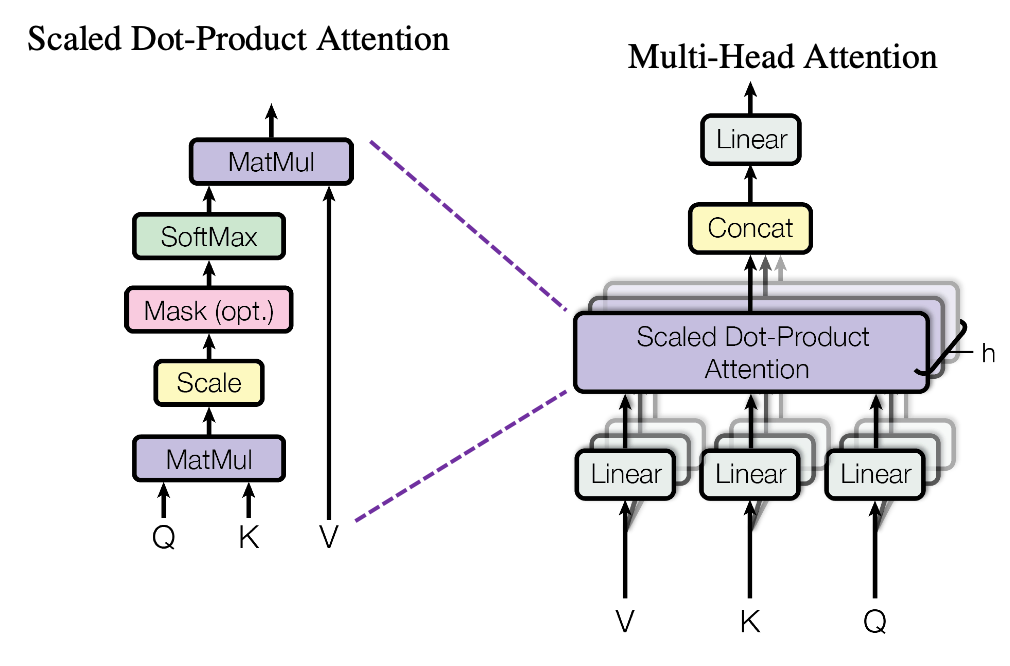
\includegraphics{./Images/mha_img_original.png}
\caption{Attention}
\end{figure}

\section{Multi-Head Attention}\label{multi-head-attention}

Instead of computing a single attention function, transformers use
**multi-head attention**, which allows the model to focus on
different parts of the sequence simultaneously. The attention heads are
computed as:
\[\text{MultiHead}(Q, K, V) = \text{Concat}(\text{head}_1, \text{head}_2, ..., \text{head}_h) W_O\]
where each attention head computes attention independently before being
concatenated and linearly transformed.

\chapter{Transformer Encoder Architecture}\label{transformer-encoder-architecture}

The **Transformer encoder** consists of multiple stacked layers,
each containing:

\begin{itemize}
\item
  Multi-head self-attention mechanism
\item
  Feed-forward network (FFN)
\item
  Residual connections and Layer Normalization
\end{itemize}

Each encoder block follows this sequence:

\begin{enumerate}
\def\labelenumi{\arabic{enumi}.}
\item
  Input embeddings + Positional Encoding
\item
  Multi-head self-attention
\item
  Layer Normalization
\item
  Feed-forward network
\item
  Layer Normalization (again)
\end{enumerate}

The encoder processes the input in parallel, unlike RNNs, making it more
efficient for long sequences.

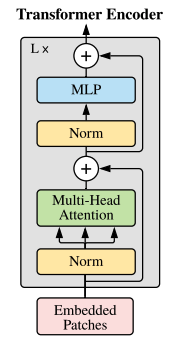
\includegraphics{./Images/TRANSFORMER ENCORDER.png}
\#\# Input to Transformers

There transformer models consist of the following inputs

\begin{enumerate}
\def\labelenumi{\arabic{enumi}.}
\tightlist
\item
  Token Embedding generated using word2vec or similar word embeddings
\item
  Segment Embedding
\item
  Position Embedding
\end{enumerate}

\begin{figure}
\centering
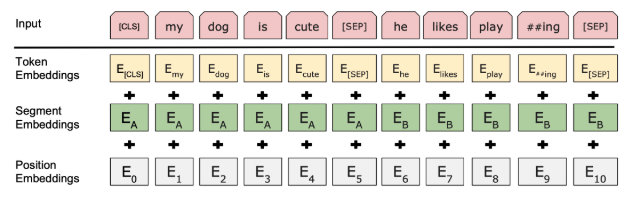
\includegraphics{./Images/BERT_INPUT.png}
\caption{Input to transformer}
\end{figure}

\section{Transformer Architectures: BERT vs.~GPT vs.~Encoder-Decoder Models}\label{transformer-architectures-bert-vs.-gpt-vs.-encoder-decoder-models}

Transformer models revolutionized deep learning by replacing RNNs and CNNs in NLP tasks. The core difference between BERT, GPT, and Encoder-Decoder models lies in how they use the Transformer components: encoder, decoder, or both.

\begin{figure}
\centering
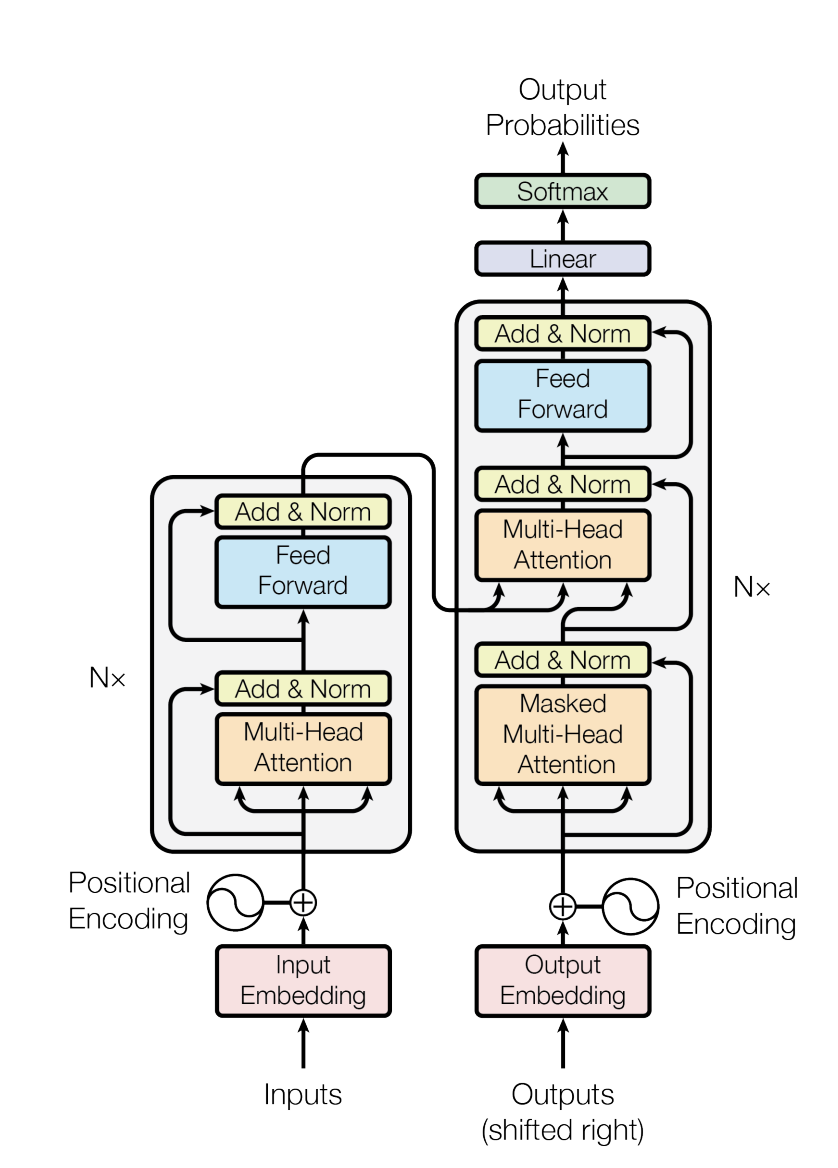
\includegraphics{./Images/Transformer_arch.png}
\caption{Transformer}
\end{figure}

\section{Masked Language Modeling (MLM)}\label{masked-language-modeling-mlm}

MLM is commonly used in natural language processing (NLP) tasks, where a
fraction of the input tokens are randomly masked, and the model learns
to predict the missing tokens based on their context. The objective
function for MLM is:
\[\mathcal{L}_{MLM} = - \sum_{i \in M} \log P(x_i | x_{\backslash i})\]
where \(M\) represents the set of masked positions, and
\(P(x_i | x_{\backslash i})\) is the probability of correctly predicting
the masked token.

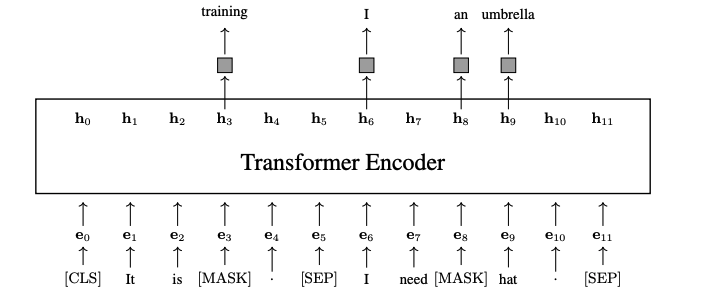
\includegraphics{./Images/MASK_LM.png}
\#\#Decorder Models (e.g.~GPT)

GPT is a decorder model

\section{Encoder Decorder Models (e.g.~BERT)}\label{encoder-decorder-models-e.g.-bert}

BERT IS and example of encoder decorder model

\section{Summary of key of transformer Archtecture}\label{summary-of-key-of-transformer-archtecture}

\section{Model Comparison}\label{model-comparison}

\begin{longtable}[]{@{}
  >{\raggedright\arraybackslash}p{(\columnwidth - 6\tabcolsep) * \real{0.2160}}
  >{\raggedright\arraybackslash}p{(\columnwidth - 6\tabcolsep) * \real{0.2560}}
  >{\raggedright\arraybackslash}p{(\columnwidth - 6\tabcolsep) * \real{0.2320}}
  >{\raggedright\arraybackslash}p{(\columnwidth - 6\tabcolsep) * \real{0.2960}}@{}}
\toprule\noalign{}
\begin{minipage}[b]{\linewidth}\raggedright
Feature
\end{minipage} & \begin{minipage}[b]{\linewidth}\raggedright
BERT 🟢 (Encoder-Only)
\end{minipage} & \begin{minipage}[b]{\linewidth}\raggedright
GPT 🔴 (Decoder-Only)
\end{minipage} & \begin{minipage}[b]{\linewidth}\raggedright
Encoder-Decoder 🔵 (T5, BART, etc.)
\end{minipage} \\
\midrule\noalign{}
\endhead
\bottomrule\noalign{}
\endlastfoot
\textbf{Architecture} & Encoder-only & Decoder-only & Both Encoder \& Decoder \\
\textbf{Directionality} & Bidirectional & Unidirectional (left-to-right) & Bidirectional encoding, left-to-right decoding \\
\textbf{Training Objective} & MLM (Masked Language Model) & CLM (Causal Language Model) & Various (e.g., seq-to-seq, denoising) \\
\textbf{Main Usage} & Understanding & Generation & Translation, Summarization \\
\end{longtable}

\chapter{Vision Transformers (ViTs)}\label{vision-transformers-vits}

ViTs apply **self-attention** to image data, treating images as
sequences of patches rather than using convolutional operations.

\begin{figure}
\centering
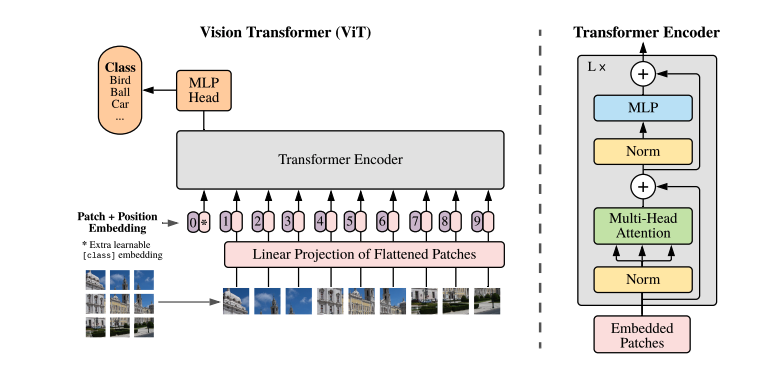
\includegraphics{./Images/Vision Transformer .png}
\caption{VISION TRANFORMER}
\end{figure}

\section{Patch Extraction and Encoding}\label{patch-extraction-and-encoding}

An image is split into patches, flattened, and passed through a
**linear projection**: \[X_{patch} = W_E \cdot X_{input} + b_E\]
where \(W_E\) is the embedding matrix and \(b_E\) is a bias term. These
embeddings are then processed using self-attention layers to extract
contextual information.

\chapter{Contrastive Language-Image Pretraining (CLIP)}\label{contrastive-language-image-pretraining-clip}

CLIP is a multimodal self-supervised learning model designed to learn
joint representations of images and text. It is trained on a large
dataset of image-text pairs using a contrastive learning approach.

\section{Architecture}\label{architecture}

CLIP consists of two main components:

\begin{itemize}
\item
  An image encoder (ResNet or Vision Transformer)
\item
  A text encoder (Transformer-based model)
\end{itemize}

Both encoders project images and text into a shared embedding space,
where semantically similar images and text have higher similarity
scores.

\begin{figure}
\centering
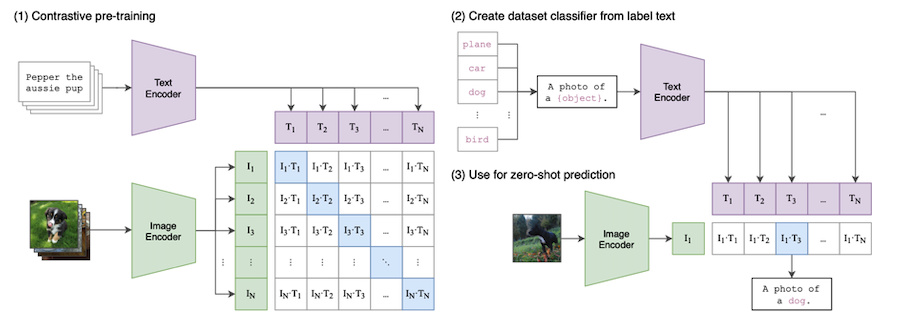
\includegraphics{./Images/CLIP.png}
\caption{CLIP Model}
\end{figure}

\section{Training Objective}\label{training-objective}

CLIP uses a contrastive learning objective where it maximizes the cosine
similarity between matching image-text pairs while minimizing similarity
between mismatched pairs:
\[\mathcal{L}_{CLIP} = - \sum_{i} \log \frac{e^{\cos(I_i, T_i)/\tau}}{\sum_j e^{\cos(I_i, T_j)/\tau}}\]
where \(I_i\) and \(T_i\) are corresponding image-text pairs, and \(\tau\) is
a temperature parameter that controls the sharpness of the distribution.

\section{Applications of CLIP}\label{applications-of-clip}

\begin{itemize}
\item
  Zero-shot image classification
\item
  Image retrieval and search
\item
  Generating text-based descriptions of images
\item
  Few-shot learning for downstream vision tasks
\end{itemize}

CLIP's ability to understand images and text jointly makes it a powerful
model for many vision-language applications.

\chapter{DINO: Self-Supervised Vision Encoding}\label{dino-self-supervised-vision-encoding}

DINO (Self-Distillation without Labels) is a **self-supervised
learning method** that trains a **student** network to predict the
output of a momentum **teacher** network.

\begin{figure}
\centering
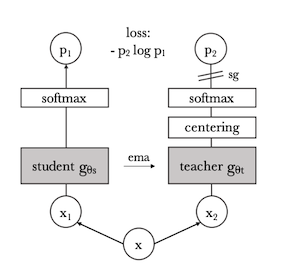
\includegraphics{./Images/DINO.png}
\caption{ENCODER}
\end{figure}

\section{Key Features of DINO}\label{key-features-of-dino}

\begin{itemize}
\item
  Works with both CNNs and ViTs
\item
  Learns representations using **contrastive learning**
\item
  Uses a momentum teacher-student setup
\item
  Multi-crop augmentation for efficient feature learning
\item
  Achieves competitive performance in unsupervised representation
  learning
\end{itemize}

\section{DINO Training Process}\label{dino-training-process}

The DINO training process uses a self-supervised learning (SSL) approach that can be interpreted as a form of knowledge distillation without labels. It involves a student network and a teacher network that have the same architecture but different parameters. The key steps in the DINO training process are as follows:

•Input and Augmentation: An input image is passed through two different random transformations, creating two distorted views. These views are fed into the student and teacher networks.

•Student and Teacher Networks: The student network (gθs) and the teacher network (gθt) process the augmented images, outputting feature maps. The teacher network's output is centered by subtracting the mean over the batch. Both the student's and teacher's outputs are normalized using a softmax function with a temperature parameter that controls the output distribution.

•Loss Calculation: A cross-entropy loss is calculated by measuring the similarity between the probability distributions from the student network and the teacher network. The student network is trained to match the output of the teacher network using this loss function.DINO minimizes the cross-entropy loss between teacher and student
outputs: \[\mathcal{L}_{DINO} = - \sum_{i} p_i^T \log p_i^S\] where
\(p_i^T\) and \(p_i^S\) are teacher and student predictions.

•Teacher Update: The teacher network's parameters are updated using an exponential moving average (EMA) of the student network's parameters. Gradient back-propagation is limited to the student network. The teacher network is updated by the formula: c ← mc+ (1−m) 1/B * ∑(from i=1 to B) gθt(xi), where `m' is a rate parameter and `B' is the batch size.

•Centering and Sharpening: The teacher network's output is centered with a mean computed over the batch, and output sharpening is achieved by using a low temperature value in the teacher's softmax normalisation.

•Multi-Crop Training: The student is fed multiple crops of an image, and it must align its local feature representations with those predicted by the teacher network for the global views of the image. This helps the network learn distinctive local features required for tasks like semantic segmentation.

•Momentum Encoder: The momentum teacher constantly outperforms the student during training. This is achieved by updating the teacher parameters using an exponential moving average of the student's parameters. The momentum encoder helps to stabilise training and improves performance.

•Multi-crop Augmentation: Training with multiple crops of an image improves performance. DINO benefits significantly from multi-crop training.

•Cross-Entropy Loss: Using a cross-entropy loss on the sharpened softmax outputs is an important component for good features.

•Centering: Centering the teacher output is important in avoiding collapse, particularly when a predictor or batch normalisation is not used.

The DINO framework is flexible and works on both convolutional neural networks (convnets) and Vision Transformers (ViTs) without modifying the architecture or internal normalisations

\chapter{DINOv2: Improved Vision Encoding}\label{dinov2-improved-vision-encoding}

DINOv2 extends DINO with **Masked Image Modeling (MIM)** and
**Self-Supervised Instance Discrimination**, improving its ability
to capture both local and global features.

\section{Key Improvements in DINOv2}\label{key-improvements-in-dinov2}

\begin{itemize}
\item
  Introduces **masked image modeling (MIM)** to learn local
  textures
\item
  Uses **multi-crop augmentation** to enhance representation
  learning
\item
  No reliance on **text supervision** (unlike CLIP)
\item
  Improved transferability to **dense prediction tasks** (e.g.,
  segmentation)
\item
  Asymmetric teacher-student design for more effective training
\item
  Incorporates KoLeo regularization to improve feature uniformity
\end{itemize}

\section{Masked Image Modeling (MIM)}\label{masked-image-modeling-mim}

MIM extends the concept of MLM to images by randomly masking patches in
an image and training the model to reconstruct the missing information.
The objective function for MIM is:
\[\mathcal{L}_{MIM} = - \sum_{i \in M} \log P(I_i | I_{\backslash i})\]
where \(I_i\) represents the masked image patch, and \(I_{\backslash i}\)
denotes the observed patches.

\section{Training Objectives}\label{training-objectives}

DINOv2 uses a **hybrid objective**:
\[\mathcal{L}_{DINOv2} = \lambda_1 \mathcal{L}_{MIM} + \lambda_2 \mathcal{L}_{Instance}\]
where:

\begin{itemize}
\item
  \(\mathcal{L}_{MIM}\) is the loss for **masked image modeling**,
  focusing on reconstructing masked patches
\item
  \(\mathcal{L}_{Instance}\) is the loss for **instance
  discrimination**, ensuring robust feature alignment across
  augmentations
\end{itemize}

DINOv2 leverages a **vision-only training approach**, making it
highly effective for self-supervised learning in image-based tasks.

\section{Applications of DINO}\label{applications-of-dino}

DINO and DINOv2 represent significant advances in **self-supervised
learning for vision tasks**. Their ability to learn rich
representations **without labeled data** makes them valuable for
diverse applications such as **image classification, retrieval,
segmentation, and biomedical imaging**.

Some applications of DINO include:

•Image Classification: DINO can be used for image classification tasks, achieving high accuracy on benchmarks such as ImageNet. It has been shown to outperform other self-supervised methods when used with ViTs. For example, DINO achieves 80.1\% top-1 accuracy on ImageNet in linear evaluation with ViT-Base, which is superior to previous self-supervised features.

•Feature Extraction: DINO can extract robust visual features that are useful for various downstream tasks. These features capture semantic information about the image, and are effective when used in combination with k-NN classifiers. DINO features have demonstrated excellent k-NN classification performance. For example, a ViT-S/8 trained with DINO reached 78.3\% top-1 accuracy on ImageNet with a k-NN classifier.

•Object Discovery and Segmentation: Self-supervised ViT features from DINO contain explicit information about the semantic segmentation of an image. This is a unique property that is not as apparent with supervised ViTs or with convnets. DINO trained ViTs are able to separate objects.

•Image Retrieval: DINO features can be used for image retrieval tasks. DINO outperforms supervised learning methods in image retrieval tasks. When trained on the Google Landmarks v2 (GLDv2) dataset, DINO ViT features perform exceptionally well for landmark retrieval.

•Copy Detection: DINO can be applied to copy detection tasks where the goal is to identify images that have been distorted. ViTs trained with DINO are very competitive in this application.

•Transfer Learning: Features pre-trained with DINO transfer effectively to various downstream tasks, outperforming supervised pre-training in many cases. Fine-tuning DINO pre-trained models on downstream tasks leads to improved results compared to models trained with supervision. Self-supervised pre-training with DINO significantly improves results on ImageNet, achieving 1-2\% improvement over supervised pre-training.

•Low-shot learning: DINO can be used for low-shot learning, where models are trained with very little labelled data. DINO has shown strong performance in low-shot learning scenarios.

•Medical Imaging: The DINO framework can be adapted for medical imaging applications. RAD-DINO, a model pre-trained using the DINOv2 framework, demonstrates that high-quality biomedical image encoders can be trained using only unimodal imaging data, without relying on text supervision. This is especially useful where there is a scarcity of paired image-text data. RAD-DINO performs comparably or better than state-of-the-art language-supervised models on image classification, semantic segmentation, and text report generation from images.

◦Image classification RAD-DINO achieves similar or superior performance levels on image classification tasks compared to language-supervised models.

◦Semantic segmentation RAD-DINO performs well on semantic segmentation tasks without needing large, densely annotated training datasets.

◦Report generation RAD-DINO excels at generating accurate text reports from images, outperforming models trained with language supervision.

◦Prediction of demographic information RAD-DINO can more accurately predict patient demographic information (e.g., sex or age) compared to language-supervised models.

\chapter{GENERATIVE MODELS}\label{generative-models}

\chapter{GENERATIVE MODEL}\label{generative-model}

\#\#GAN

\chapter{Introduction to GAN Models}\label{introduction-to-gan-models}

Generative Adversarial Networks (GANs) are a class of machine learning models that consist of two neural networks, a generator and a discriminator, which are trained simultaneously through a game-theoretic framework. The generator creates data that resembles a target distribution, while the discriminator attempts to distinguish between real data and data generated by the generator.

\section{GAN Architecture}\label{gan-architecture}

A GAN consists of two main components:
- \textbf{Generator} \(G\): Generates synthetic data samples.
- \textbf{Discriminator} \(D\): Distinguishes between real and generated data samples.

\subsection{Objective}\label{objective}

The objective of a GAN is to train both the generator and the discriminator such that the generator learns to generate data that is indistinguishable from real data.

Let:
- \(x\) be the real data.
- \(G(z)\) be the generated data, where \(z\) is the input to the generator (typically noise).
- \(D(x)\) be the probability that \(x\) is real, i.e., \(D(x) = P(\text{real}|x)\).
- \(D(G(z))\) be the probability that \(G(z)\) is real, i.e., \(D(G(z)) = P(\text{real}|G(z))\).

\subsection{Discriminator Loss}\label{discriminator-loss}

The discriminator tries to maximize the probability of correctly distinguishing real and fake data. The objective function for the discriminator is:

\[
\mathcal{L}_D = -\mathbb{E}_{x \sim p_{\text{data}}(x)}[\log D(x)] - \mathbb{E}_{z \sim p_z(z)}[\log(1 - D(G(z)))]
\]

Where:
- \(p_{\text{data}}(x)\) is the distribution of real data.
- \(p_z(z)\) is the distribution of noise (input to the generator).

The first term encourages the discriminator to assign high probability to real data, and the second term encourages the discriminator to assign low probability to fake data generated by the generator.

\subsection{Generator Loss}\label{generator-loss}

The generator tries to fool the discriminator by generating data that is classified as real. The objective function for the generator is:

\[
\mathcal{L}_G = -\mathbb{E}_{z \sim p_z(z)}[\log D(G(z))]
\]

The generator minimizes the log of the discriminator's output, meaning it aims to generate data that the discriminator will classify as real.

\subsection{Minimax Game}\label{minimax-game}

The overall GAN training objective is a minimax game between the generator and the discriminator:

\[
\min_G \max_D \mathcal{L}(D, G) = \mathbb{E}_{x \sim p_{\text{data}}(x)}[\log D(x)] + \mathbb{E}_{z \sim p_z(z)}[\log(1 - D(G(z)))]
\]

The generator \(G\) tries to minimize this loss, while the discriminator \(D\) tries to maximize it.

\section{Training GANs}\label{training-gans}

The GAN model is trained using the following procedure:
1. \textbf{Train the discriminator} \(D\) to maximize \(\mathcal{L}_D\), i.e., improve its ability to distinguish between real and fake data.
2. \textbf{Train the generator} \(G\) to minimize \(\mathcal{L}_G\), i.e., improve its ability to generate data that the discriminator classifies as real.
3. Repeat the process iteratively until both the generator and the discriminator converge.

\section{Key GAN Model Architectures}\label{key-gan-model-architectures}

GANs are powerful models for generating synthetic data, with applications in image generation, video generation, and other domains. However, training GANs is challenging, as it requires balancing the generator and discriminator to ensure they both improve simultaneously. Generative Adversarial Networks (GANs) have evolved significantly since their introduction. Various architectures have been proposed to enhance performance in different tasks such as image generation, super-resolution, and style transfer. Below, we review some of the key GAN architectures and their strengths and limitations.

\section{1. Vanilla GAN}\label{vanilla-gan}

The Vanilla GAN is the original GAN model introduced by Ian Goodfellow and his collaborators in 2014. It consists of a simple architecture with a generator \(G\) and a discriminator \(D\), both of which are fully connected neural networks.

\subsection{Pros:}\label{pros}

\begin{itemize}
\tightlist
\item
  Simple and easy to understand.
\item
  Good for basic GAN tasks with simple datasets.
\item
  Serves as the foundation for more advanced GAN architectures.
\end{itemize}

\subsection{Cons:}\label{cons}

\begin{itemize}
\tightlist
\item
  Prone to training instability.
\item
  Difficulty in capturing complex data distributions.
\item
  Mode collapse: The generator may produce limited variety in outputs.
\end{itemize}

\section{2. Deep Convolutional GAN (DCGAN)}\label{deep-convolutional-gan-dcgan}

DCGAN, introduced by Radford et al.~(2015), is a modification of the Vanilla GAN that uses deep convolutional networks in both the generator and the discriminator. It leverages convolutional layers to capture spatial hierarchies in data, particularly for image generation tasks.

\subsection{Pros:}\label{pros-1}

\begin{itemize}
\tightlist
\item
  Works well for generating high-quality images.
\item
  Stability improvements over the Vanilla GAN due to the use of convolutional layers.
\item
  Better handling of spatial data and images.
\end{itemize}

\subsection{Cons:}\label{cons-1}

\begin{itemize}
\tightlist
\item
  Requires large amounts of data to train effectively.
\item
  Still vulnerable to mode collapse in some cases.
\item
  May struggle with high-dimensional data.
\end{itemize}

\section{3. Conditional GAN (CGAN)}\label{conditional-gan-cgan}

Conditional GANs, introduced by Mirza and Osindero (2014), condition both the generator and the discriminator on some additional information, such as labels or attributes. This allows the model to generate specific outputs conditioned on input variables.

\subsection{Pros:}\label{pros-2}

\begin{itemize}
\tightlist
\item
  Enables conditional image generation (e.g., generating images of a specific class).
\item
  Better control over the outputs.
\item
  Can be used for tasks like image-to-image translation.
\end{itemize}

\subsection{Cons:}\label{cons-2}

\begin{itemize}
\tightlist
\item
  Requires labeled data for training.
\item
  May suffer from overfitting if not properly regularized.
\item
  Can still experience training instability.
\end{itemize}

\section{4. Wasserstein GAN (WGAN)}\label{wasserstein-gan-wgan}

WGAN, introduced by Arjovsky et al.~(2017), modifies the loss function of the GAN to use the Wasserstein distance (also known as Earth-Mover's Distance) instead of the standard Jensen-Shannon divergence. This leads to improved training stability.

\subsection{Pros:}\label{pros-3}

\begin{itemize}
\tightlist
\item
  Provides a more stable training process compared to Vanilla GANs.
\item
  Easier to train with fewer hyperparameter tuning requirements.
\item
  Can generate high-quality images with less likelihood of mode collapse.
\end{itemize}

\subsection{Cons:}\label{cons-3}

\begin{itemize}
\tightlist
\item
  Requires weight clipping or gradient penalty, which can be difficult to implement.
\item
  Slightly slower to train compared to other models due to the optimization of Wasserstein distance.
\item
  Limited application for non-image data tasks.
\end{itemize}

\section{5. CycleGAN}\label{cyclegan}

CycleGAN, introduced by Zhu et al.~(2017), is designed for image-to-image translation tasks without requiring paired training data. It leverages cycle consistency to ensure that an image generated by transforming from domain A to domain B can be transformed back to domain A, preserving its content.

\subsection{Pros:}\label{pros-4}

\begin{itemize}
\tightlist
\item
  Enables image-to-image translation without paired data.
\item
  Effective for tasks like style transfer and photo enhancement.
\item
  Flexible and widely applicable for unpaired image datasets.
\end{itemize}

\subsection{Cons:}\label{cons-4}

\begin{itemize}
\tightlist
\item
  Requires a large amount of training data.
\item
  May produce blurry or low-quality images compared to supervised models.
\item
  Can be computationally expensive and hard to train.
\end{itemize}

\section{6. Progressive GAN (ProGAN)}\label{progressive-gan-progan}

Progressive GANs, introduced by Karras et al.~(2018), address the problem of training deep networks by progressively growing both the generator and discriminator. The model starts by training on low-resolution images and gradually increases the resolution during the training process.

\subsection{Pros:}\label{pros-5}

\begin{itemize}
\tightlist
\item
  Generates high-resolution and highly realistic images.
\item
  Reduces the complexity of training by starting with simpler models.
\item
  Stable training process compared to traditional GANs.
\end{itemize}

\subsection{Cons:}\label{cons-5}

\begin{itemize}
\tightlist
\item
  Training can be slow as it requires progressively growing the network.
\item
  Computationally expensive, especially for high-resolution outputs.
\item
  Not ideal for tasks that require real-time or fast inference.
\end{itemize}

\section{7. StyleGAN}\label{stylegan}

StyleGAN, introduced by Karras et al.~(2019), extends the idea of progressive training by introducing a new architecture where the generator uses a ``style'' vector to control different levels of detail in the generated images, such as coarse features, textures, and fine details.

\subsection{Pros:}\label{pros-6}

\begin{itemize}
\tightlist
\item
  State-of-the-art in generating high-quality, realistic images, particularly faces.
\item
  Excellent control over the generated image's style and attributes.
\item
  Capable of generating extremely high-resolution images.
\end{itemize}

\subsection{Cons:}\label{cons-6}

\begin{itemize}
\tightlist
\item
  Extremely computationally expensive to train.
\item
  Requires large datasets for meaningful results.
\item
  Complex architecture, making it harder to implement and understand.
\end{itemize}

\section{Summary}\label{summary}

Each GAN architecture has its strengths and weaknesses, and the choice of which one to use depends on the specific task and the dataset at hand. While models like DCGAN and WGAN are more stable for general tasks, others like CycleGAN and StyleGAN excel in specific applications such as image translation and high-quality image generation. Careful consideration of the pros and cons is essential to selecting the right model for a given problem.

\section{Variational Autoencoders (VAEs)}\label{variational-autoencoders-vaes}

Variational Autoencoders (VAEs) are a class of deep generative models that use variational inference to learn a probabilistic mapping from data to a latent space. A key component of VAEs is the \textbf{Kullback-Leibler (KL) Divergence}, which acts as a regularization term to ensure that the learned latent distribution is close to a predefined prior distribution.

In this, we will:
- Define KL divergence mathematically.
- Use KL divergence to derive the \textbf{VAE loss function}.
- Explain the \textbf{VAE architecture} and how it works.

\begin{center}\rule{0.5\linewidth}{0.5pt}\end{center}

\chapter{2. Kullback-Leibler (KL) Divergence}\label{kullback-leibler-kl-divergence}

\subsection{\texorpdfstring{\textbf{Definition}}{Definition}}\label{definition}

KL Divergence measures the difference between two probability distributions. Given two distributions:
- \(P(x)\) (true distribution)
- \(Q(x)\) (approximate distribution),

the KL divergence is defined as:

\[
D_{KL}( Q(x) || P(x) ) = \sum_x Q(x) \log \frac{Q(x)}{P(x)}
\]

or in the continuous case:

\[
D_{KL}( Q(x) || P(x) ) = \int Q(x) \log \frac{Q(x)}{P(x)} dx
\]

\begin{itemize}
\tightlist
\item
  If \(Q(x)\) is the same as \(P(x)\), then \(D_{KL} = 0\) (no divergence).
\item
  Otherwise, it quantifies how much \(Q(x)\) differs from \(P(x)\).
\item
  KL divergence is \textbf{not symmetric}, meaning \(D_{KL}(Q||P) \neq D_{KL}(P||Q)\).
\end{itemize}

\begin{center}\rule{0.5\linewidth}{0.5pt}\end{center}

\chapter{3. Derivation of the VAE Loss Function}\label{derivation-of-the-vae-loss-function}

Variational Autoencoders aim to learn a probabilistic mapping from input data \(x\) to a latent space represented by a \textbf{latent variable} \(z\). Instead of encoding each \(x\) deterministically, VAEs \textbf{model the latent space as a probability distribution}.

\subsection{\texorpdfstring{\textbf{Bayesian Formulation in VAEs}}{Bayesian Formulation in VAEs}}\label{bayesian-formulation-in-vaes}

We define:
- \(p(x)\) → True data distribution (unknown)
- \(p(z)\) → Prior over latent space (typically a normal distribution: \(N(0, I)\))
- \(p(x | z)\) → Likelihood (decoder)
- \(q(z | x)\) → Posterior approximation (encoder)

The goal of training a VAE is to maximize the likelihood:

\[
\log p(x)
\]

Since computing \(p(x)\) directly is intractable, we introduce a variational approximation using \textbf{ELBO (Evidence Lower Bound)}.

\[
\log p(x) = D_{KL} ( q(z | x) || p(z | x) ) + \mathbb{E}_{q(z|x)} [\log p(x | z)]
\]

Rearranging:

\[
\log p(x) - D_{KL} ( q(z | x) || p(z | x) ) = \mathbb{E}_{q(z|x)} [\log p(x | z)] - D_{KL}(q(z | x) || p(z))
\]

Since KL divergence is always \textbf{non-negative}, the right-hand side forms a lower bound:

\[
\mathcal{L}_{ELBO} = \mathbb{E}_{q(z|x)} [\log p(x | z)] - D_{KL}(q(z | x) || p(z))
\]

This \textbf{ELBO loss function} balances two terms:
1. \textbf{Reconstruction Loss} \(\mathbb{E}_{q(z|x)} [\log p(x | z)]\): Ensures generated samples resemble real data.
2. \textbf{KL Divergence} \(D_{KL}(q(z | x) || p(z))\): Encourages the latent distribution to stay close to the prior (e.g., normal distribution \(N(0, I)\)).

The final \textbf{VAE loss function} is:

\[
\mathcal{L} = - \mathbb{E}_{q(z|x)} [\log p(x | z)] + D_{KL}(q(z | x) || p(z))
\]

\begin{center}\rule{0.5\linewidth}{0.5pt}\end{center}

\chapter{4. Variational Autoencoder (VAE) Architecture}\label{variational-autoencoder-vae-architecture}

\subsection{\texorpdfstring{\textbf{VAE Structure}}{VAE Structure}}\label{vae-structure}

A VAE consists of two networks:

\begin{enumerate}
\def\labelenumi{\arabic{enumi}.}
\item
  \textbf{Encoder (Inference Network)}

  \begin{itemize}
  \tightlist
  \item
    Maps input \(x\) to latent distribution parameters \(\mu\) and \(\sigma\).
  \item
    Approximates \(q(z | x) = N(\mu(x), \sigma^2(x)I)\).
  \end{itemize}
\item
  \textbf{Latent Space Sampling}

  \begin{itemize}
  \tightlist
  \item
    Instead of directly sampling from \(q(z | x)\), we use the \textbf{reparameterization trick}:
  \end{itemize}

  \[
  z = \mu + \sigma \cdot \epsilon, \quad \epsilon \sim N(0, I)
  \]

  This enables gradient-based optimization.
\item
  \textbf{Decoder (Generative Network)}

  \begin{itemize}
  \tightlist
  \item
    Maps latent variable \(z\) back to data space.
  \item
    Models likelihood \(p(x | z)\).
  \end{itemize}
\end{enumerate}

\section{Summary}\label{summary-1}

\begin{itemize}
\tightlist
\item
  KL Divergence ensures that the learned latent space distribution
  𝑞(𝑧∣𝑥) stays close to a prior distribution p(z).
\item
  VAE optimizes ELBO, balancing reconstruction loss (data fidelity) and KL loss (latent regularization).
\item
  Reparameterization trick enables training via backpropagation.
\end{itemize}

Key references

\begin{enumerate}
\def\labelenumi{\arabic{enumi}.}
\tightlist
\item
  Kingma, D.P., \& Welling, M. (2013). ``Auto-Encoding Variational Bayes.''
\item
  Doersch, C. (2016). ``Tutorial on Variational Autoencoders.''
\end{enumerate}

\chapter{Why the Field Moved Away from VAEs and GANs}\label{why-the-field-moved-away-from-vaes-and-gans}

Generative modeling has evolved rapidly over the past decade, with models like Variational Autoencoders (VAEs) and Generative Adversarial Networks (GANs) playing a major role. However, researchers have increasingly shifted focus to other models due to the limitations of VAEs and GANs. Below, we explore why the field has moved away from these models and what newer approaches have emerged.

\section{1. Issues with GANs (Generative Adversarial Networks)}\label{issues-with-gans-generative-adversarial-networks}

\subsection{a. Training Instability}\label{a.-training-instability}

\begin{itemize}
\tightlist
\item
  \textbf{Mode Collapse}: GANs are prone to mode collapse, where the generator produces limited, repetitive outputs. This happens when the generator finds a small subset of outputs that the discriminator incorrectly classifies as real.
\item
  \textbf{Vanishing Gradients}: The adversarial loss function used by GANs can lead to vanishing gradients, especially when the discriminator becomes too strong relative to the generator.
\item
  \textbf{Difficulty in Convergence}: GANs often struggle with convergence, as both the generator and discriminator need to improve at the same rate, which can be difficult to balance.
\end{itemize}

\subsection{b. Lack of Good Evaluation Metrics}\label{b.-lack-of-good-evaluation-metrics}

\begin{itemize}
\tightlist
\item
  Unlike VAEs, which have a clear likelihood-based objective, GANs lack a standard method to evaluate the quality of the generated samples. Traditional metrics like Inception Score (IS) and Fréchet Inception Distance (FID) are limited in assessing the true diversity and realism of the outputs.
\end{itemize}

\subsection{c.~Training Challenges}\label{c.-training-challenges}

\begin{itemize}
\tightlist
\item
  \textbf{Adversarial Nature}: GANs involve a delicate balance between the generator and discriminator. This adversarial setup is sensitive to hyperparameter choices and can lead to training instability, requiring careful tuning to prevent one network from overpowering the other.
\end{itemize}

\section{2. Issues with VAEs (Variational Autoencoders)}\label{issues-with-vaes-variational-autoencoders}

\subsection{a. Blurry Outputs}\label{a.-blurry-outputs}

\begin{itemize}
\tightlist
\item
  \textbf{Mode Averaging}: VAEs tend to produce blurry outputs because they average over all possible outputs for a given input, as part of the variational inference process. This results in images that lack sharpness and fine details, especially in high-resolution tasks.
\end{itemize}

\subsection{b. Poorly Structured Latent Space}\label{b.-poorly-structured-latent-space}

\begin{itemize}
\tightlist
\item
  \textbf{Latent Space Limitations}: Despite the VAE objective encouraging a regularized latent space, it doesn't always guarantee that the latent variables will be disentangled or meaningfully aligned with the semantics of the data. This leads to suboptimal latent space representations.
\end{itemize}

\subsection{c.~Inconsistent Trade-Off Between Terms}\label{c.-inconsistent-trade-off-between-terms}

\begin{itemize}
\tightlist
\item
  The VAE objective function consists of a reconstruction term and a regularization term (KL-divergence), which enforces a prior distribution on the latent variables. Balancing these two terms can be difficult, and improper balancing can result in poor generative performance or overfitting.
\end{itemize}

\section{3. Shift Towards New Models}\label{shift-towards-new-models}

\subsection{a. Flow-Based Models (Normalizing Flows)}\label{a.-flow-based-models-normalizing-flows}

\begin{itemize}
\tightlist
\item
  Flow-based models, like RealNVP and Glow, allow for exact likelihood estimation and have been used to generate high-quality samples. These models invert the generative process, which isn't possible with GANs and VAEs.
\end{itemize}

\subsubsection{Pros:}\label{pros-7}

\begin{itemize}
\tightlist
\item
  Exact log-likelihood computation.
\item
  Better sample quality and sharper images than VAEs.
\end{itemize}

\subsubsection{Cons:}\label{cons-7}

\begin{itemize}
\tightlist
\item
  High computational cost, both during training and inference.
\item
  Requires reversible transformations, which can be challenging to implement.
\end{itemize}

\subsection{b. Autoregressive Models (PixelCNN, PixelSNAIL)}\label{b.-autoregressive-models-pixelcnn-pixelsnail}

\begin{itemize}
\tightlist
\item
  Autoregressive models generate data one pixel at a time (or one point in sequence) by modeling the joint probability of the data. They have been highly effective for image generation and other structured data tasks.
\end{itemize}

\subsubsection{Pros:}\label{pros-8}

\begin{itemize}
\tightlist
\item
  High-quality, sharp images.
\item
  Strong performance in tasks like image denoising and inpainting.
\end{itemize}

\subsubsection{Cons:}\label{cons-8}

\begin{itemize}
\tightlist
\item
  Slow inference speed since they generate data sequentially.
\item
  High computational cost during inference.
\end{itemize}

\subsection{c.~Transformers for Generation}\label{c.-transformers-for-generation}

\begin{itemize}
\tightlist
\item
  Transformers, initially used for NLP, have been adapted for image generation tasks (e.g., DALL-E, Vision Transformers). These models excel in scalability and generalization across different data types.
\end{itemize}

\subsubsection{Pros:}\label{pros-9}

\begin{itemize}
\tightlist
\item
  State-of-the-art performance on large datasets.
\item
  Flexible for multimodal tasks, including text and image generation.
\end{itemize}

\subsubsection{Cons:}\label{cons-9}

\begin{itemize}
\tightlist
\item
  Requires large datasets and computational resources.
\item
  Inference can be slow, especially with large models.
\end{itemize}

\subsection{d.~Score-based Models (Denoising Diffusion Probabilistic Models)}\label{d.-score-based-models-denoising-diffusion-probabilistic-models}

\begin{itemize}
\tightlist
\item
  Denoising Diffusion Probabilistic Models (DDPM) have gained traction due to their ability to generate high-quality samples with less likelihood of mode collapse compared to GANs.
\end{itemize}

\subsubsection{Pros:}\label{pros-10}

\begin{itemize}
\tightlist
\item
  High-quality samples with sharp details and diversity.
\item
  Better robustness to mode collapse.
\end{itemize}

\subsubsection{Cons:}\label{cons-10}

\begin{itemize}
\tightlist
\item
  Slow generation process due to multiple diffusion steps.
\item
  Computationally expensive, especially for high-dimensional data.
\end{itemize}

\section{4. Why the Shift?}\label{why-the-shift}

\subsection{a. Better Evaluation and Stability}\label{a.-better-evaluation-and-stability}

\begin{itemize}
\tightlist
\item
  Newer models like flow-based models and score-based models offer stability and a clear evaluation framework, which is crucial for reliable performance in generative tasks.
\end{itemize}

\subsection{b. Improved Sample Quality}\label{b.-improved-sample-quality}

\begin{itemize}
\tightlist
\item
  Models like diffusion models provide sharper and higher-quality samples, addressing the blurry outputs of VAEs and the mode collapse issues of GANs.
\end{itemize}

\subsection{c.~Scalability and Flexibility}\label{c.-scalability-and-flexibility}

\begin{itemize}
\tightlist
\item
  Transformer-based models and flow-based models are highly scalable and flexible, capable of handling diverse data types, including images, text, and even multimodal data. This has made them more versatile for a variety of generative tasks.
\end{itemize}

\section{Conclusion}\label{conclusion-1}

While VAEs and GANs were groundbreaking when introduced, newer generative models such as flow-based models, autoregressive models, and diffusion models offer significant improvements in terms of training stability, sample quality, and scalability. These advancements have led to a shift in focus within the generative modeling community, as they better address the limitations of VAEs and GANs. However, VAEs and GANs still serve as foundational models and remain useful in specific tasks where their strengths are beneficial.

\chapter{DIFFUSION MODELS}\label{diffusion-models}

\section{1. Introduction to DDPMs}\label{introduction-to-ddpms}

Denoising Diffusion Probabilistic Models (DDPMs) are a class of \textbf{generative models} that gradually transform noise into meaningful data through a \textbf{reverse diffusion process}. Unlike Variational Autoencoders (VAEs) or Generative Adversarial Networks (GANs), DDPMs model the data distribution by progressively \textbf{adding and removing noise} in a \textbf{Markovian fashion}.

\begin{itemize}
\tightlist
\item
  \textbf{Forward process:} Gradually adds noise to input data \(x_0\), making it resemble pure Gaussian noise.
\item
  \textbf{Reverse process:} Learns to remove noise step-by-step to recover the original data.
\end{itemize}

This process is governed by KL divergence, leading to a well-defined \textbf{variational lower bound (ELBO)} loss function.

\begin{center}\rule{0.5\linewidth}{0.5pt}\end{center}

\section{2. Mathematical Formulation of Diffusion Models}\label{mathematical-formulation-of-diffusion-models}

Let \(x_0\) be a sample from the data distribution \(q(x_0)\). The goal is to model \(p_\theta(x_0)\), which generates realistic samples.

\section{\texorpdfstring{\textbf{2.1 Forward Diffusion Process}}{2.1 Forward Diffusion Process}}\label{forward-diffusion-process}

The forward diffusion process \textbf{corrupts} the data by adding Gaussian noise at each time step \(t\):

\[
q(x_t | x_{t-1}) = \mathcal{N}(x_t ; \sqrt{1 - \beta_t} x_{t-1}, \beta_t I)
\]

where:
- \(\beta_t\) is a \textbf{variance schedule} that controls noise addition.
- \(x_t\) is the intermediate noisy image.

By iterating over many steps, \(x_T\) approaches a Gaussian distribution:

\[
q(x_T) \approx \mathcal{N}(0, I)
\]

We can directly sample \(x_t\) at any time step using:

\[
q(x_t | x_0) = \mathcal{N}(x_t ; \sqrt{\bar{\alpha}_t} x_0, (1 - \bar{\alpha}_t) I)
\]

where:

\[
\bar{\alpha}_t = \prod_{i=1}^{t} (1 - \beta_i)
\]

\begin{center}\rule{0.5\linewidth}{0.5pt}\end{center}

\section{3. Reverse Diffusion Process}\label{reverse-diffusion-process}

The goal is to \textbf{reverse the forward process} by learning \(p_\theta(x_{t-1} | x_t)\):

\[
p_\theta(x_{t-1} | x_t) = \mathcal{N}(x_{t-1} ; \mu_\theta(x_t, t), \Sigma_\theta(x_t, t))
\]

\begin{itemize}
\tightlist
\item
  \(\mu_\theta(x_t, t)\) is a neural network predicting the denoised sample.
\item
  \(\Sigma_\theta(x_t, t)\) represents learned variance.
\end{itemize}

This step gradually \textbf{removes noise}, reconstructing the original image.

\begin{center}\rule{0.5\linewidth}{0.5pt}\end{center}

\section{4. Derivation of the DDPM Loss Function Using KL Divergence}\label{derivation-of-the-ddpm-loss-function-using-kl-divergence}

To train a DDPM, we \textbf{maximize the likelihood} of the data \(p_\theta(x_0)\). Since direct computation is intractable, we \textbf{optimize the Evidence Lower Bound (ELBO)}:

\[
\log p_\theta(x_0) \geq \mathbb{E}_{q(x_{1:T} | x_0)} \left[ \log \frac{p_\theta(x_0:T)}{q(x_{1:T} | x_0)} \right]
\]

Expanding the ELBO:

\[
\mathcal{L}_{ELBO} = \mathbb{E}_q \left[ D_{KL} (q(x_T | x_0) || p(x_T)) + \sum_{t=1}^{T} D_{KL} (q(x_{t-1} | x_t, x_0) || p_\theta(x_{t-1} | x_t)) \right]
\]

\subsection{\texorpdfstring{\textbf{Key Terms in the Loss Function}}{Key Terms in the Loss Function}}\label{key-terms-in-the-loss-function}

\begin{enumerate}
\def\labelenumi{\arabic{enumi}.}
\item
  \textbf{Final Step KL Term} \(D_{KL} (q(x_T | x_0) || p(x_T))\):

  \begin{itemize}
  \tightlist
  \item
    Since \(x_T\) is already close to \(\mathcal{N}(0, I)\), this term \textbf{vanishes}.
  \end{itemize}
\item
  \textbf{Reconstruction Loss} (Mean Squared Error Formulation):

  \begin{itemize}
  \tightlist
  \item
    Instead of directly minimizing KL divergence, we rewrite the KL term in terms of \textbf{noise prediction}:
  \end{itemize}

  \[
  \mathbb{E}_{x_0, \epsilon} \left[ \|\epsilon - \epsilon_\theta(x_t, t)\|^2 \right]
  \]

  where:

  \begin{itemize}
  \tightlist
  \item
    \(\epsilon \sim \mathcal{N}(0, I)\) is the true noise added to the data.
  \item
    \(\epsilon_\theta(x_t, t)\) is the predicted noise by the model.
  \end{itemize}
\end{enumerate}

\subsection{\texorpdfstring{\textbf{Final DDPM Loss Function}}{Final DDPM Loss Function}}\label{final-ddpm-loss-function}

\[
\mathcal{L} = \mathbb{E}_{t, x_0, \epsilon} \left[ w_t \|\epsilon - \epsilon_\theta(x_t, t)\|^2 \right]
\]

where \(w_t\) is an optional weighting factor.

This means DDPMs \textbf{learn to predict the noise}, making the model \textbf{denoise data at every step}.

To understand the optimizing objective of diffusion models please read:

\url{https://jehillparikh.medium.com/understanding-diffusion-models-optimization-objective-d7214d36dbd8}
Optimizing the Reverse Process Covariance
To train DDPMs with a learned reverse process covariance, Σθ, the full KL divergence term needs to be optimised9. One approach, as described in10, is to:
1.Train the noise prediction network, εθ, using Lsimple.
2.Train Σθ using the full KL divergence-based loss function.
Generating New Samples
Once the DDPM is trained, new images can be generated by starting with random noise, xT \textasciitilde{} N(0, I), at the final timestep T, and iteratively sampling xt-1 from the learned reverse process pθ(xt-1\textbar xt) until reaching x09. Each sampling step utilises the reparameterisation trick to draw samples from the conditional Gaussian distribution.
Advantages of DDPMs
●High Sample Quality: DDPMs are known for generating high-quality samples, often surpassing the visual fidelity of samples produced by GANs.
●Stability and Ease of Training: DDPM training is generally more stable than adversarial training used in GANs.
Limitations of DDPMs
●Computational Cost: The iterative nature of both the forward and reverse processes can be computationally expensive, especially for high-resolution images.
●Slow Sampling: Generating samples using the iterative reverse process can be slow, requiring multiple steps to obtain a final sample.

\section{IMPLEMENTATION OF DDPM}\label{implementation-of-ddpm}

Forward Process Implementation in Diffusion Models
The forward process in diffusion models involves gradually adding Gaussian noise to data samples over a series of timesteps, transforming the data distribution into a simple Gaussian distribution. The implementation of this process is straightforward and involves repeatedly sampling from Gaussian distributions with predefined variances.
The forward process is defined as a Markov chain, where each timestep t depends only on the previous timestep t-1.

At each timestep, Gaussian noise is added to the sample from the previous timestep. The variance of the added noise is typically controlled by a schedule, which can be linear, cosine, or other forms.

The forward process can be expressed mathematically as:

q(xt\textbar xt-1) = N(xt; √αtxt-1, (1 - αt)I)

where:

xt is the noisy sample at timestep t.
αt is a hyperparameter that determines the variance of the Gaussian noise added at timestep t. It is typically a decreasing function of t, meaning that more noise is added in the early timesteps.
I is the identity matrix.

The forward process can be implemented efficiently using the reparameterization trick, which allows sampling from the Gaussian distribution by transforming a sample from a standard normal distribution.

By repeatedly applying the forward process, the data distribution is gradually transformed into a Gaussian distribution with mean 0 and variance 1.

The number of timesteps in the forward process is a hyperparameter that affects the quality of the generated samples and the computational cost of training and sampling

This to sample a noisy image at time T without needing a neural network.

Practical Considerations
Noise Schedule: The choice of noise schedule significantly impacts the training and sampling efficiency of diffusion models. Different noise schedules can lead to variations in sample quality and convergence speed.

Number of Timesteps: A larger number of timesteps generally result in a smoother transition to the Gaussian noise distribution but increase the computational cost.

Computational Efficiency: The forward process is computationally efficient as it only involves sampling from Gaussian distributions. However, the computational cost increases linearly with the number of timesteps.

Data Preprocessing: In practice, the input data might be preprocessed before applying the forward process, such as normalisation or resizing, depending on the specific task and dataset.

\section{Learning the Reverse Process in Diffusion Models}\label{learning-the-reverse-process-in-diffusion-models}

Diffusion models are trained to learn a reverse process that gradually removes the noise added during the forward process, ultimately generating new data samples. This reverse process is modelled as a series of denoising steps, each aiming to recover a slightly less noisy sample from the previous timestep. The success of diffusion models hinges on effectively learning this reverse denoising process.
●The reverse process is modelled as a Markov chain, similar to the forward process, but operating in reverse time order.
●The model learns to predict the conditional probability distribution of a less noisy sample, xt-1, given a noisy sample, xt, from the previous timestep.
●This conditional probability distribution is typically modelled as a Gaussian distribution:
●pθ(xt-1\textbar xt) = N(µθ(xt), Σθ(xt))
●where:
○µθ(xt) is the predicted mean of the distribution, representing the denoised sample.
○Σθ(xt) is the predicted covariance matrix, capturing the uncertainty in the denoising process.
○θ represents the model parameters.

The model architecture, often a U-Net or a Diffusion Transformer (DiT), is trained to predict the parameters of this Gaussian distribution.
●Training Objective: The model is trained to minimise the difference between the predicted noise and the ground truth noise added during the forward process. This can be achieved using various objective functions, including mean squared error (MSE) or variational lower bounds on the data likelihood.

\section{UNETS}\label{unets}

The U-Net architecture consists of an encoder and a decoder pathway connected by skip connections.2
○The encoder pathway downsamples the input image, extracting features at different resolutions.2
○The decoder pathway upsamples the encoded features, reconstructing the image at the original resolution.2
○The skip connections transfer features from the encoder to the decoder at corresponding resolutions, enabling the model to preserve fine-grained details and capture both local and global image information.2
●In diffusion models, the U-Net takes a noisy image sample, xt, and its corresponding timestep, t, as input and predicts the noise added to the image or the denoised image, xt-1.2
●U-Nets for diffusion models often incorporate additional components, such as attention mechanisms and adaptive normalisation layers, to improve performance and enable conditioning on external information.2
○Attention mechanisms allow the model to selectively focus on specific regions of the image, enhancing its ability to capture complex relationships and generate high-quality samples.2
○Adaptive normalisation layers, such as Adaptive Layer Normalisation (adaLN), enable the model to condition on external information, such as class labels or text prompts, by modulating the normalisation process based on this information.234 This allows for controlled generation of samples that adhere to specific constraints or conditions.
FOR MODEL DETAILS SEE BLOG POST AND REFERENCE WITHIN

\url{https://jehillparikh.medium.com/u-nets-with-attention-c8d7e9bf2416}

\chapter{1. Introduction to Score-Based Generative Models (SGMs)}\label{introduction-to-score-based-generative-models-sgms}

Score-Based Generative Models (SGMs), also called \textbf{Score Matching with Langevin Dynamics (SMLD)} or \textbf{Denoising Score Matching (DSM)}, are a class of diffusion models that \textbf{learn the score function} (gradient of the log-likelihood) to generate realistic data.

Unlike \textbf{Denoising Diffusion Probabilistic Models (DDPMs)}, which define the process discretely, SGMs generalize diffusion models using \textbf{Stochastic Differential Equations (SDEs)} for continuous noise perturbation.

\subsection{\texorpdfstring{\textbf{Key Properties}}{Key Properties}}\label{key-properties}

\begin{itemize}
\tightlist
\item
  Forward process transforms data into Gaussian noise.
\item
  Reverse process learns to \textbf{estimate the score function} \(\nabla_x \log p_t(x)\).
\item
  Uses \textbf{Score Matching Loss} derived from KL divergence.
\end{itemize}

\begin{center}\rule{0.5\linewidth}{0.5pt}\end{center}

\chapter{2. Mathematical Formulation of Score-Based Models}\label{mathematical-formulation-of-score-based-models}

Let \(x_0 \sim p(x)\) be a real data sample. The \textbf{goal} is to model the distribution \(p(x)\) by learning its \textbf{score function} \(s_\theta(x_t, t)\).

\subsection{\texorpdfstring{\textbf{2.1 Forward Process: Stochastic Differential Equation (SDE)}}{2.1 Forward Process: Stochastic Differential Equation (SDE)}}\label{forward-process-stochastic-differential-equation-sde}

SGMs define a \textbf{continuous diffusion process} via an \textbf{SDE}:

\[
dx = f(x, t) dt + g(t) dW
\]

where:
- \(W\) is a \textbf{Wiener process} (Brownian motion).
- \(f(x, t)\) is the drift coefficient.
- \(g(t)\) is the diffusion coefficient.
- The noise gradually transforms \(x_0\) into pure Gaussian noise.

Common \textbf{SDE choices}:
1. \textbf{Variance-Preserving (VP) SDE} (similar to DDPM):
\[
   dx = -\frac{1}{2} \beta_t x dt + \sqrt{\beta_t} dW
   \]
2. \textbf{Variance-Exploding (VE) SDE}:
\[
   dx = \sqrt{\frac{d[\sigma^2(t)]}{dt}} dW
   \]

where \(\sigma^2(t)\) controls noise addition.

At large \(t\), \(x_t\) becomes Gaussian:

\[
q(x_t | x_0) = \mathcal{N}(x_t ; x_0 e^{-\frac{1}{2} \beta_t}, (1 - e^{-\beta_t}) I)
\]

\begin{center}\rule{0.5\linewidth}{0.5pt}\end{center}

\chapter{3. Reverse Process: Score-Based Generative Model}\label{reverse-process-score-based-generative-model}

To \textbf{generate data}, we \textbf{reverse the SDE}:

\[
dx = [f(x,t) - g(t)^2 \nabla_x \log p_t(x)] dt + g(t) dW
\]

Instead of modeling \(p_t(x)\), we approximate the \textbf{score function}:

\[
s_\theta(x_t, t) \approx \nabla_x \log p_t(x)
\]

Thus, the reverse process \textbf{gradually denoises samples from Gaussian noise}.

\begin{center}\rule{0.5\linewidth}{0.5pt}\end{center}

\chapter{4. Derivation of the Score-Based Loss Function Using KL Divergence}\label{derivation-of-the-score-based-loss-function-using-kl-divergence}

Since direct optimization of likelihood is intractable, we use the \textbf{KL divergence between forward and reverse processes}.

\[
\mathcal{L} = \mathbb{E}_q \left[ D_{KL} (q(x_T | x_0) || p(x_T)) + \int_0^T D_{KL} (q(x_{t-1} | x_t, x_0) || p_\theta(x_{t-1} | x_t)) dt \right]
\]

Since \(q(x_T) \approx \mathcal{N}(0, I)\), the first term vanishes.

Using \textbf{Score Matching}, we rewrite KL as:

\[
\mathcal{L}_{score} = \mathbb{E}_{t, x_t} \left[ w(t) \| s_\theta(x_t, t) - \nabla_x \log q(x_t | x_0) \|^2 \right]
\]

where \(w(t)\) is a weighting function.

\subsection{\texorpdfstring{\textbf{Final Score Matching Loss}}{Final Score Matching Loss}}\label{final-score-matching-loss}

\[
\mathcal{L}_{score} = \mathbb{E}_{t, x_t} \left[ \| s_\theta(x_t, t) - \frac{x_t - x_0}{\sigma_t^2} \|^2 \right]
\]

SGMs train by \textbf{matching the estimated score function to the true score}.

\begin{center}\rule{0.5\linewidth}{0.5pt}\end{center}

Score-based diffusion models are another prominent class of diffusion models. They are based on the concept of ``scores,'' which are the gradients of the log-probability density function of the data distribution. These models learn to estimate the score of the data distribution at different noise levels and then use Langevin dynamics, a sampling method based on stochastic differential equations, to generate new samples.
Score Estimation: A key component of score-based models is estimating the score function at various noise levels. This is typically done by training a neural network to predict the score of a noisy data sample given its noise level.

Annealed Langevin Dynamics: During sampling, annealed Langevin dynamics is employed to generate samples. This iterative process starts with a sample from a prior distribution and then repeatedly updates the sample by moving it in the direction of the estimated score function, adding noise, and gradually decreasing the noise level over time.
Diffusion models IN score based generative models as introduced by Song et al

Score-based generative models, a category that encompasses diffusion models, represent probability distributions through their score functions. The score function is a vector field that points in the direction of the steepest ascent of the log-probability density of the data distribution. This means it indicates the direction in which the likelihood of the data increases most rapidly.

A key advantage of using score functions is that they can be learned from data without requiring adversarial optimisation, unlike models like Generative Adversarial Networks (GANs). This makes training score-based models potentially simpler and more stable.

Score-based models learn the score function by training a neural network, called the score network, to denoise images corrupted with Gaussian noise. This process involves perturbing data with Gaussian noise at multiple scales to enable the network to capture both coarse-grained and fine-grained image features.

Once the score network is trained, new samples can be generated by employing a process called Langevin dynamics. Langevin dynamics is a sampling method that iteratively refines a sample by using the score function to guide it towards regions of higher probability density.

This procedure begins with an initial sample of white noise and gradually denoises it into an image using the learned score network. The iterative updates in Langevin dynamics can be viewed as noisy gradient ascent on the log-density of the data distribution.

A challenge in training score-based models is determining the appropriate noise scales to use during training. Choosing the right noise scales is critical for the success of these models, as using a single noise scale can lead to poor sample quality, particularly for large images.

Intuitively, high noise levels aid in estimating the score function but result in corrupted samples, while low noise levels produce cleaner samples but make score function estimation more difficult. To balance these trade-offs, score-based models typically leverage multiple noise scales.

Another technique proposed in the source is the use of an exponential moving average (EMA) of model parameters to improve stability during training. This technique has been shown to effectively stabilise training, reduce artifacts in generated samples, and ultimately lead to better FID scores.

Although score-based models have a unified training objective and don't require adversarial training, they can exhibit instability in generated image quality, especially for higher-resolution images. EMA helps mitigate this issue.
Here is a detailed explanation of the training and sampling process for score-based models, based on the information provided in the sources:
Training Score-Based Models
Objective: The primary goal of training a score-based model is to learn the score function of the data distribution. The score function, denoted as ∇x log p(x), represents the gradient of the log-probability density function of the data distribution, p(x). This function essentially indicates the direction in which the data distribution's likelihood increases most rapidly.

Score Network: A neural network, called the score network, is trained to approximate this score function. This network takes a data sample, x, as input and outputs a vector that estimates the score at that point.

Denoising Score Matching: A common method for training the score network is denoising score matching (DSM). This approach involves perturbing the training data with Gaussian noise at different scales and training the score network to denoise these corrupted samples.

The training objective in DSM is to minimise the difference between the predicted score by the score network and the true score of the perturbed data distribution. This objective encourages the network to learn how to accurately estimate the score function across various noise levels.

Perturbation with Multiple Noise Scales: Using multiple noise scales during training is crucial for the success of score-based models. High noise levels help estimate the score function at a coarse level, capturing the overall structure of the data distribution, while low noise levels refine the score estimation in the high-density regions, enhancing the fidelity of the generated samples.

Song et al emphasizes the importance of choosing appropriate noise scales and proposes techniques for analytically determining an effective set of noise scales based on the training data. This approach helps to automate the process of noise scale selection, improving training efficiency and model performance.

Noise Conditional Score Network (NCSN): To handle multiple noise scales effectively, a specific architecture called a Noise Conditional Score Network (NCSN) is often employed. This network takes both the data sample, x, and the noise level, σ, as inputs and outputs the estimated score at that point.

The song et al introduces an efficient NCSN parameterization where the score function is computed as sθ(x, σ) = sθ(x)/ σ, where sθ(x) is an unconditional score network. This method simplifies the implementation and can handle many noise scales, even continuous ones, effectively.
Sampling from Score-Based Models
Langevin Dynamics: Once the score network is trained, it can be used to generate new samples from the learned data distribution. This generation process typically involves a sampling technique called Langevin dynamics.

Langevin dynamics is an iterative process that starts with an initial sample, typically drawn from a simple noise distribution like a Gaussian. The score function, as estimated by the trained score network, is then used to guide the sample towards regions of higher probability density in the data distribution.

Annealed Langevin Dynamics: In practice, a variant called annealed Langevin dynamics is often employed. This approach involves sampling from a series of perturbed data distributions with decreasing noise levels. This gradual decrease in noise levels helps the sampling process converge more effectively to the target data distribution.

Annealed Langevin dynamics as a method that combines information from all noise scales, starting from the largest noise scale and progressively refining the samples by moving to smaller scales.

Iterative Refinement: At each step of Langevin dynamics, the current sample is updated by taking a small step in the direction indicated by the score function, with an added noise term. This noise term introduces stochasticity into the sampling process, helping to explore different regions of the data distribution and preventing the samples from getting stuck in local optima.

As the process progresses, the influence of the noise term diminishes, and the samples gradually converge to the target data distribution, guided by the score function.

Parameter Configuration: The effectiveness of annealed Langevin dynamics heavily relies on properly setting parameters like the number of sampling steps per noise scale, T, and the step size parameter, ε.

Song et al provides theoretically motivated guidance for configuring these parameters, aiming to optimise the performance of annealed Langevin dynamics without relying on extensive manual tuning.

Additional Considerations
Exponential Moving Average (EMA): The source ``2006.09011v2.pdf'' also highlights the use of an exponential moving average (EMA) of the score network's parameters during training. EMA helps to stabilize the training process, especially for high-resolution image generation, where the model might exhibit unstable behaviour despite the unified training objective.

EMA involves maintaining a weighted average of the model's parameters over the training iterations, with more recent parameters receiving higher weights. This averaging process helps to smooth out fluctuations in the parameter updates, leading to a more stable training trajectory and reducing artifacts in the generated samples.

\chapter{\texorpdfstring{\textbf{Chapter: Reinforcement Learning - Theory and Applications}}{Chapter: Reinforcement Learning - Theory and Applications}}\label{chapter-reinforcement-learning---theory-and-applications}

\section{\texorpdfstring{\textbf{1. Introduction}}{1. Introduction}}\label{introduction-2}

Reinforcement Learning (RL) is a subfield of machine learning that deals with sequential decision-making problems. Unlike supervised learning, where labeled data is used for training, RL agents learn by interacting with the environment through trial and error to maximize a long-term objective, often represented as cumulative rewards.

RL has been widely applied in various domains, including robotics, finance, healthcare, and gaming. The ability of RL to handle complex, dynamic environments makes it a powerful paradigm for artificial intelligence research and real-world applications.

\section{\texorpdfstring{\textbf{2. Fundamentals of Reinforcement Learning}}{2. Fundamentals of Reinforcement Learning}}\label{fundamentals-of-reinforcement-learning}

\subsection{\texorpdfstring{\textbf{2.1 Key Components of RL}}{2.1 Key Components of RL}}\label{key-components-of-rl}

\begin{enumerate}
\def\labelenumi{\arabic{enumi}.}
\tightlist
\item
  \textbf{Agent}: The entity that makes decisions and interacts with the environment.
\item
  \textbf{Environment}: The external system with which the agent interacts.
\item
  \textbf{State (s)}: A representation of the environment at a specific time.
\item
  \textbf{Action (a)}: A decision taken by the agent that affects the environment.
\item
  \textbf{Reward (r)}: A scalar value that provides feedback on the effectiveness of an action.
\item
  \textbf{Policy (π)}: A strategy mapping states to actions.
\item
  \textbf{Value Function (V(s))}: The expected cumulative reward starting from state \emph{s} and following policy \emph{π}.
\item
  \textbf{Q-Function (Q(s, a))}: The expected cumulative reward for taking action \emph{a} in state \emph{s} and following policy \emph{π} thereafter.
\item
  \textbf{Discount Factor (γ)}: A factor that determines the importance of future rewards, where \emph{0 ≤ γ ≤ 1}.
\end{enumerate}

\subsection{\texorpdfstring{\textbf{2.2 The RL Process}}{2.2 The RL Process}}\label{the-rl-process}

The RL process can be mathematically formulated as a Markov Decision Process (MDP), defined by the tuple (\emph{S, A, P, R, γ}), where:
- \emph{S} is the set of possible states.
- \emph{A} is the set of possible actions.
- \emph{P(s'\textbar s,a)} is the transition probability from state \emph{s} to \emph{s'} given action \emph{a}.
- \emph{R(s,a)} is the reward function.
- \emph{γ} is the discount factor.

The goal of RL is to find an optimal policy \emph{π} that maximizes expected cumulative reward.

\section{\texorpdfstring{\textbf{3. Types of Reinforcement Learning}}{3. Types of Reinforcement Learning}}\label{types-of-reinforcement-learning}

\subsection{\texorpdfstring{\textbf{3.1 Model-Based vs Model-Free RL}}{3.1 Model-Based vs Model-Free RL}}\label{model-based-vs-model-free-rl}

\begin{itemize}
\tightlist
\item
  \textbf{Model-Based RL}: The agent builds an internal model of the environment and uses it to make decisions.
\item
  \textbf{Model-Free RL}: The agent learns through direct interaction without explicit modeling.
\end{itemize}

\subsection{\texorpdfstring{\textbf{3.2 Value-Based vs Policy-Based RL}}{3.2 Value-Based vs Policy-Based RL}}\label{value-based-vs-policy-based-rl}

\begin{itemize}
\tightlist
\item
  \textbf{Value-Based RL}: Focuses on learning the value function (e.g., Q-learning, DQN).
\item
  \textbf{Policy-Based RL}: Directly optimizes the policy function (e.g., REINFORCE algorithm).
\item
  \textbf{Actor-Critic Methods}: Combines value-based and policy-based approaches (e.g., A2C, PPO).
\end{itemize}

\section{\texorpdfstring{\textbf{4. Popular RL Algorithms}}{4. Popular RL Algorithms}}\label{popular-rl-algorithms}

\subsection{\texorpdfstring{\textbf{4.1 Q-Learning}}{4.1 Q-Learning}}\label{q-learning}

Q-learning is a model-free, off-policy algorithm that updates Q-values using the Bellman equation:

\begin{Shaded}
\begin{Highlighting}[]
\NormalTok{Q(s, a) = Q(s, a) + \textbackslash{}alpha [r + \textbackslash{}gamma \textbackslash{}max\_\{a\textquotesingle{}\} Q(s\textquotesingle{}, a\textquotesingle{}) {-} Q(s, a)]}
\end{Highlighting}
\end{Shaded}

where \emph{α} is the learning rate and \emph{γ} is the discount factor.

\subsection{\texorpdfstring{\textbf{4.2 Q-Learning Policy Gradient Theorem}}{4.2 Q-Learning Policy Gradient Theorem}}\label{q-learning-policy-gradient-theorem}

The policy gradient theorem states that the gradient of the expected cumulative reward with respect to policy parameters is:

\begin{Shaded}
\begin{Highlighting}[]
\NormalTok{\textbackslash{}nabla\_\textbackslash{}theta J(\textbackslash{}theta) = \textbackslash{}mathbb\{E\}\_\{\textbackslash{}pi\} \textbackslash{}left[ \textbackslash{}nabla\_\textbackslash{}theta \textbackslash{}log \textbackslash{}pi\_\textbackslash{}theta(a|s) Q\^{}\{\textbackslash{}pi\}(s, a) \textbackslash{}right]}
\end{Highlighting}
\end{Shaded}

This theorem serves as the foundation of policy gradient methods, which optimize policies directly.

\subsection{\texorpdfstring{\textbf{4.3 Deep Q-Networks (DQN)}}{4.3 Deep Q-Networks (DQN)}}\label{deep-q-networks-dqn}

DQN extends Q-learning by utilizing deep neural networks to approximate the Q-function. It stabilizes training through experience replay and a target network.

\subsection{\texorpdfstring{\textbf{4.4 Policy Gradient Methods}}{4.4 Policy Gradient Methods}}\label{policy-gradient-methods}

Policy gradient methods optimize the policy directly using gradient ascent:

\begin{Shaded}
\begin{Highlighting}[]
\NormalTok{\textbackslash{}nabla\_\textbackslash{}theta J(\textbackslash{}theta) = \textbackslash{}mathbb\{E\}[\textbackslash{}nabla\_\textbackslash{}theta \textbackslash{}log \textbackslash{}pi\_\textbackslash{}theta(a|s) R]}
\end{Highlighting}
\end{Shaded}

Examples: REINFORCE, A2C, PPO

\section{\texorpdfstring{\textbf{5. Applications of Reinforcement Learning}}{5. Applications of Reinforcement Learning}}\label{applications-of-reinforcement-learning}

\begin{itemize}
\tightlist
\item
  \textbf{Robotics}: Training autonomous robots for navigation and manipulation.
\item
  \textbf{Gaming}: Mastering complex games like Go (AlphaGo), StarCraft (AlphaStar), and Poker.
\item
  \textbf{Finance}: Algorithmic trading, portfolio optimization.
\item
  \textbf{Healthcare}: Optimizing treatment strategies and drug discovery.
\item
  \textbf{Industrial Automation}: Smart manufacturing and supply chain optimization.
\end{itemize}

\section{\texorpdfstring{\textbf{6. Challenges in RL}}{6. Challenges in RL}}\label{challenges-in-rl}

\begin{itemize}
\tightlist
\item
  \textbf{Exploration vs Exploitation Tradeoff}: Balancing between trying new actions and maximizing known rewards.
\item
  \textbf{Sample Inefficiency}: RL models require extensive interaction data.
\item
  \textbf{Sparse Rewards}: Some environments provide infrequent feedback.
\item
  \textbf{Stability and Convergence Issues}: RL algorithms can be unstable and require extensive tuning.
\item
  \textbf{Generalization}: Transferring learned policies to new environments remains challenging.
\end{itemize}

\section{\texorpdfstring{\textbf{7. Conclusion and Future Directions}}{7. Conclusion and Future Directions}}\label{conclusion-and-future-directions}

Reinforcement Learning is a rapidly evolving field with growing applications across industries. Future research aims to address sample inefficiency, stability, and generalization while exploring novel architectures such as meta-learning and self-supervised RL.

\begin{center}\rule{0.5\linewidth}{0.5pt}\end{center}

\emph{For further reading, consider Sutton \& Barto's ``Reinforcement Learning: An Introduction'' and recent advancements in deep RL research papers.}

\chapter{\texorpdfstring{\textbf{Markov Decision Process (MDP)}}{Markov Decision Process (MDP)}}\label{markov-decision-process-mdp}

A \textbf{Markov Decision Process (MDP)} is a framework for modeling decision-making where outcomes are partly random and partly controlled by an agent. MDPs are widely used in \textbf{reinforcement learning (RL), robotics, finance, and game theory}.

An MDP consists of the following components:

\begin{itemize}
\tightlist
\item
  \textbf{States (\(S\)):} A set of all possible states the agent can be in.
\item
  \textbf{Actions (\(A\)):} A set of all possible actions the agent can take.
\item
  \textbf{Transition Probability (\(P\)):} The probability of moving from one state to another given an action.
\item
  \textbf{Reward Function (\(R\)):} The reward received for taking an action in a particular state.
\item
  \textbf{Policy (\(\pi\)):} A strategy that defines the action selection process in each state.
\item
  \textbf{Discount Factor (\(\gamma\)):} A factor that determines how much future rewards are valued compared to immediate rewards.
\end{itemize}

Mathematically, an MDP is represented as a tuple:

\begin{Shaded}
\begin{Highlighting}[]
\NormalTok{(S, A, P, R, \textbackslash{}pi, \textbackslash{}gamma)}
\end{Highlighting}
\end{Shaded}

where:

\begin{itemize}
\tightlist
\item
  \(S\) is the set of states.
\item
  \(A\) is the set of actions.
\item
  \(P(s' | s, a)\) is the probability of transitioning from state \(s\) to state \(s'\) when taking action \(a\).
\item
  \(R(s, a)\) is the reward received after taking action \(a\) in state \(s\).
\item
  \(\pi(a | s)\) is the policy, which defines the probability of taking action \(a\) in state \(s\).
\item
  \(\gamma \in [0,1]\) is the discount factor.
\end{itemize}

\section{\texorpdfstring{\textbf{State Transition Probability}}{State Transition Probability}}\label{state-transition-probability}

The probability of moving from state \(s\) to state \(s'\) after taking action \(a\) is given by:

\begin{Shaded}
\begin{Highlighting}[]
\NormalTok{P(s\textquotesingle{} | s, a) = \textbackslash{}Pr(S\_\{t+1\} = s\textquotesingle{} | S\_t = s, A\_t = a)}
\end{Highlighting}
\end{Shaded}

This represents the \textbf{Markov Property}, meaning the next state \textbf{only depends on the current state and action}, not the previous history.

\begin{center}\rule{0.5\linewidth}{0.5pt}\end{center}

\section{\texorpdfstring{\textbf{Policy in MDP}}{Policy in MDP}}\label{policy-in-mdp}

A \textbf{policy (\(\pi\))} defines the agent's behavior by mapping states to actions. Policies can be:

\begin{itemize}
\item
  \textbf{Deterministic Policy (\(\pi: S \to A\))}: The agent always takes a specific action in a given state.

\begin{Shaded}
\begin{Highlighting}[]
\NormalTok{a = \textbackslash{}pi(s)}
\end{Highlighting}
\end{Shaded}
\item
  \textbf{Stochastic Policy (\(\pi: S \times A \to [0,1]\))}: The agent chooses actions probabilistically.

\begin{Shaded}
\begin{Highlighting}[]
\NormalTok{\textbackslash{}pi(a | s) = \textbackslash{}Pr(A\_t = a | S\_t = s)}
\end{Highlighting}
\end{Shaded}
\end{itemize}

\section{\texorpdfstring{\textbf{Optimal Policy (\(\pi^*\))}}{Optimal Policy (\textbackslash pi\^{}*)}}\label{optimal-policy-pi}

An optimal policy \(\pi^*\) maximizes the expected return:

\begin{Shaded}
\begin{Highlighting}[]
\NormalTok{\textbackslash{}pi\^{}* = \textbackslash{}arg\textbackslash{}max\_\textbackslash{}pi V\^{}\textbackslash{}pi(s), \textbackslash{}forall s \textbackslash{}in S}
\end{Highlighting}
\end{Shaded}

where \(V^\pi(s)\) is the value function under policy \(\pi\). The optimal policy leads to the highest cumulative rewards over time.

\begin{center}\rule{0.5\linewidth}{0.5pt}\end{center}

\section{\texorpdfstring{\textbf{Bellman Equation}}{Bellman Equation}}\label{bellman-equation}

The \textbf{Bellman Equation} provides a recursive formula for \textbf{value functions}, helping determine the \textbf{optimal policy} that maximizes expected cumulative rewards.

\section{\texorpdfstring{\textbf{State-Value Function (\(V(s)\))}}{State-Value Function (V(s))}}\label{state-value-function-vs}

The \textbf{value function} of a state \(s\) under a policy \(\pi\) is:

\begin{Shaded}
\begin{Highlighting}[]
\NormalTok{V\^{}\textbackslash{}pi(s) = \textbackslash{}mathbb\{E\} \textbackslash{}left[ \textbackslash{}sum\_\{t=0\}\^{}\{\textbackslash{}infty\} \textbackslash{}gamma\^{}t R\_t \textbackslash{}mid S\_0 = s, \textbackslash{}pi \textbackslash{}right]}
\end{Highlighting}
\end{Shaded}

Using the \textbf{Bellman equation}, we express the recursive relationship:

\begin{Shaded}
\begin{Highlighting}[]
\NormalTok{V\^{}\textbackslash{}pi(s) = \textbackslash{}sum\_\{a \textbackslash{}in A\} \textbackslash{}pi(a | s) \textbackslash{}sum\_\{s\textquotesingle{} \textbackslash{}in S\} P(s\textquotesingle{} | s, a) \textbackslash{}left[ R(s, a) + \textbackslash{}gamma V\^{}\textbackslash{}pi(s\textquotesingle{}) \textbackslash{}right]}
\end{Highlighting}
\end{Shaded}

where:

\begin{itemize}
\tightlist
\item
  \(\pi(a | s)\) is the probability of taking action \(a\) in state \(s\).
\item
  \(P(s' | s, a)\) is the probability of transitioning to state \(s'\) given state \(s\) and action \(a\).
\item
  \(R(s, a)\) is the immediate reward.
\item
  \(\gamma\) is the discount factor.
\end{itemize}

\begin{center}\rule{0.5\linewidth}{0.5pt}\end{center}

\section{\texorpdfstring{\textbf{Action-Value Function (\(Q(s, a)\))}}{Action-Value Function (Q(s, a))}}\label{action-value-function-qs-a}

The \textbf{Q-value function} measures the expected reward for taking an action \(a\) in state \(s\) and then following policy \(\pi\):

\begin{Shaded}
\begin{Highlighting}[]
\NormalTok{Q\^{}\textbackslash{}pi(s, a) = \textbackslash{}mathbb\{E\} \textbackslash{}left[ \textbackslash{}sum\_\{t=0\}\^{}\{\textbackslash{}infty\} \textbackslash{}gamma\^{}t R\_t \textbackslash{}mid S\_0 = s, A\_0 = a, \textbackslash{}pi \textbackslash{}right]}
\end{Highlighting}
\end{Shaded}

The \textbf{Bellman equation for Q-values} is:

\begin{Shaded}
\begin{Highlighting}[]
\NormalTok{Q\^{}\textbackslash{}pi(s, a) = R(s, a) + \textbackslash{}gamma \textbackslash{}sum\_\{s\textquotesingle{} \textbackslash{}in S\} P(s\textquotesingle{} | s, a) \textbackslash{}sum\_\{a\textquotesingle{} \textbackslash{}in A\} \textbackslash{}pi(a\textquotesingle{} | s\textquotesingle{}) Q\^{}\textbackslash{}pi(s\textquotesingle{}, a\textquotesingle{})}
\end{Highlighting}
\end{Shaded}

\section{\texorpdfstring{\textbf{Optimal Policy \& Bellman Optimality Equation}}{Optimal Policy \& Bellman Optimality Equation}}\label{optimal-policy-bellman-optimality-equation}

The goal of reinforcement learning is to find the \textbf{optimal policy} that maximizes the expected cumulative reward. The \textbf{Bellman optimality equation} for the optimal state-value function is:

\begin{Shaded}
\begin{Highlighting}[]
\NormalTok{V\^{}*(s) = \textbackslash{}max\_\{a \textbackslash{}in A\} \textbackslash{}sum\_\{s\textquotesingle{} \textbackslash{}in S\} P(s\textquotesingle{} | s, a) \textbackslash{}left[ R(s, a) + \textbackslash{}gamma V\^{}*(s\textquotesingle{}) \textbackslash{}right]}
\end{Highlighting}
\end{Shaded}

Similarly, the \textbf{Bellman optimality equation for Q-values} is:

\begin{Shaded}
\begin{Highlighting}[]
\NormalTok{Q\^{}*(s, a) = R(s, a) + \textbackslash{}gamma \textbackslash{}sum\_\{s\textquotesingle{} \textbackslash{}in S\} P(s\textquotesingle{} | s, a) \textbackslash{}max\_\{a\textquotesingle{} \textbackslash{}in A\} Q\^{}*(s\textquotesingle{}, a\textquotesingle{})}
\end{Highlighting}
\end{Shaded}

where:

\begin{itemize}
\tightlist
\item
  \(V^*(s)\) is the maximum possible value of state \(s\).
\item
  \(Q^*(s, a)\) is the maximum expected return for taking action \(a\) in state \(s\).
\end{itemize}

\section{\texorpdfstring{\textbf{Conclusion}}{Conclusion}}\label{conclusion-2}

Markov Decision Processes provide a structured way to \textbf{model sequential decision-making problems}, and the \textbf{Bellman equation} helps compute optimal strategies. Q-learning is a powerful method for learning action-value functions, while policy learning focuses on directly optimizing the decision-making strategy. These concepts form the foundation of \textbf{reinforcement learning algorithms}, including \textbf{value iteration, policy iteration, and deep reinforcement learning}.

\section{\texorpdfstring{\textbf{Reinforcement learning}}{Reinforcement learning}}\label{reinforcement-learning}

Building on the previous discussion of \textbf{Markov Decision Processes (MDP)} and the \textbf{Bellman Equation}, we now explore various reinforcement learning (RL) methods. RL can be broadly categorized into \textbf{Model-Based RL} and \textbf{Model-Free RL}. These methods help agents learn optimal decision-making strategies within an environment. Additionally, we will briefly cover \textbf{Reward-Based Learning, Monte Carlo Tree Search (MCTS), Proximal Policy Optimization (PPO),} and other advanced RL techniques that extend the fundamental concepts of MDPs.

\chapter{\texorpdfstring{\textbf{Reward-Based Learning}}{Reward-Based Learning}}\label{reward-based-learning}

Reward-Based Learning is a fundamental concept in reinforcement learning where an agent learns to make decisions by receiving rewards for its actions. The agent's objective is to maximize the total cumulative reward over time. The reward signal serves as feedback to guide the agent toward optimal behavior.

\section{\texorpdfstring{\textbf{Types of Rewards}}{Types of Rewards}}\label{types-of-rewards}

\begin{itemize}
\tightlist
\item
  \textbf{Immediate Rewards (\(R(s, a)\)):} A reward received immediately after taking action \(a\) in state \(s\).
\item
  \textbf{Delayed Rewards:} A reward that is given after multiple steps, requiring the agent to learn long-term strategies.
\item
  \textbf{Sparse Rewards:} Rewards that occur infrequently, making learning more challenging.
\item
  \textbf{Dense Rewards:} Frequent rewards that provide continuous feedback.
\end{itemize}

\section{\texorpdfstring{\textbf{Reward Function}}{Reward Function}}\label{reward-function}

The reward function determines the numerical value assigned to each action and state transition. It can be defined as:

\begin{Shaded}
\begin{Highlighting}[]
\NormalTok{R: S \textbackslash{}times A \textbackslash{}to \textbackslash{}mathbb\{R\}}
\end{Highlighting}
\end{Shaded}

where \(S\) is the set of states, \(A\) is the set of actions, and the function returns a scalar reward value.

\section{\texorpdfstring{\textbf{Optimizing Rewards}}{Optimizing Rewards}}\label{optimizing-rewards}

To maximize cumulative rewards, agents use \textbf{return (\(G_t\))}, which is the sum of discounted future rewards:

\begin{Shaded}
\begin{Highlighting}[]
\NormalTok{G\_t = R\_t + \textbackslash{}gamma R\_\{t+1\} + \textbackslash{}gamma\^{}2 R\_\{t+2\} + ...}
\end{Highlighting}
\end{Shaded}

where \(\gamma\) (discount factor) determines the importance of future rewards.

\section{\texorpdfstring{\textbf{Exploration vs.~Exploitation}}{Exploration vs.~Exploitation}}\label{exploration-vs.-exploitation}

Reward-Based Learning must balance:
- \textbf{Exploration:} Trying new actions to discover potentially better rewards.
- \textbf{Exploitation:} Choosing known good actions to maximize immediate rewards.

\subsection{\texorpdfstring{\textbf{Methods for Managing Exploration-Exploitation Trade-off:}}{Methods for Managing Exploration-Exploitation Trade-off:}}\label{methods-for-managing-exploration-exploitation-trade-off}

\begin{itemize}
\tightlist
\item
  \textbf{Epsilon-Greedy Strategy:} Randomly selects an action with probability \(\epsilon\), otherwise chooses the best-known action.
\item
  \textbf{Upper Confidence Bound (UCB):} Prioritizes actions with uncertain rewards.
\item
  \textbf{Thompson Sampling:} Uses probability distributions to select actions.
\end{itemize}

\chapter{\texorpdfstring{\textbf{Model-Based Reinforcement Learning}}{Model-Based Reinforcement Learning}}\label{model-based-reinforcement-learning}

Model-Based RL refers to methods where an agent \textbf{learns a model} of the environment and uses it for decision-making. This typically involves:

\begin{enumerate}
\def\labelenumi{\arabic{enumi}.}
\tightlist
\item
  \textbf{Learning the Transition Model (\(P(s' | s, a)\))}: Predicting the next state given the current state and action.
\item
  \textbf{Learning the Reward Model (\(R(s, a)\))}: Estimating the reward for taking an action in a given state.
\item
  \textbf{Planning}: Using the learned model to simulate trajectories and improve decision-making.
\end{enumerate}

\subsection{\texorpdfstring{\textbf{Popular Model-Based RL Approaches}}{Popular Model-Based RL Approaches}}\label{popular-model-based-rl-approaches}

\begin{itemize}
\tightlist
\item
  \textbf{Dynamic Programming (DP)}: Uses Bellman equations to iteratively compute value functions, assuming a known model.
\item
  \textbf{Model Predictive Control (MPC)}: Uses a learned model to simulate future states and optimize actions.
\item
  \textbf{Dyna-Q}: Combines model-free and model-based learning by integrating planning and learning.
\end{itemize}

\section{\texorpdfstring{\textbf{Monte Carlo Tree Search (MCTS)}}{Monte Carlo Tree Search (MCTS)}}\label{monte-carlo-tree-search-mcts}

MCTS is a search-based decision-making algorithm used in \textbf{game AI} and \textbf{planning problems}. It simulates future states by exploring the decision tree and backing up estimated rewards, aligning closely with \textbf{MDP planning techniques}.

In MCTS, the algorithm uses a model of the environment (specifically, the transition dynamics of states) to simulate future outcomes. During the search process, the algorithm builds a tree of possible future states, which are explored through simulations (rollouts). These simulations rely on the model to predict the outcomes of actions, and the results of the simulations are used to evaluate the best actions to take at each decision point.

The key characteristic of MCTS being model-based is that it requires knowledge of the environment's dynamics to simulate the future. This model could either be explicitly provided (like in a chess game, where the rules of the game are well-defined) or learned through interactions (as in some planning problems for robotics)

\subsection{\texorpdfstring{\textbf{MCTS Steps}}{MCTS Steps}}\label{mcts-steps}

\begin{enumerate}
\def\labelenumi{\arabic{enumi}.}
\tightlist
\item
  \textbf{Selection}: Start from the root and select the most promising node based on a strategy (e.g., Upper Confidence Bound (UCB1)).
\item
  \textbf{Expansion}: Add a new node to the tree when a promising unexplored action is found.
\item
  \textbf{Simulation (Rollout)}: Play out random simulations to estimate the value of the new state.
\item
  \textbf{Backpropagation}: Update the values of visited nodes based on the simulation outcome.
\end{enumerate}

\subsection{Steps of MCTS}\label{steps-of-mcts}

\begin{enumerate}
\def\labelenumi{\arabic{enumi}.}
\item
  \textbf{Selection}: Starting from the root node, recursively select the child node that maximizes the \textbf{Upper Confidence Bound for Trees (UCT)}.

  The UCT formula is given by:

  \[
  \text{UCT}(v) = \frac{w(v)}{n(v)} + c \sqrt{\frac{\ln N}{n(v)}}
  \]

  Where:

  \begin{itemize}
  \tightlist
  \item
    \(w(v)\) is the total reward for node \(v\).
  \item
    \(n(v)\) is the number of times node \(v\) has been visited.
  \item
    \(N\) is the number of times the parent node has been visited.
  \item
    \(c\) is the exploration constant that balances exploration and exploitation.
  \end{itemize}
\item
  \textbf{Expansion}: If the selected node is not a terminal state and has untried actions, add a new child node representing an untried action.
\item
  \textbf{Simulation (Rollout)}: Simulate a random sequence of actions from the current node until a terminal state is reached. The outcome of the simulation gives an estimate of the value of the node.

  The return from a simulation is denoted by:

  \[
  G_t = \sum_{k=t}^{T} \gamma^{k-t} R_k
  \]

  Where:

  \begin{itemize}
  \tightlist
  \item
    \(G_t\) is the total reward (return) from time \(t\) onwards.
  \item
    \(\gamma\) is the discount factor.
  \item
    \(R_k\) is the reward at time step \(k\).
  \end{itemize}
\item
  \textbf{Backpropagation}: After the simulation, backpropagate the results by updating the values and visit counts of all nodes in the path from the current node to the root.

  The update rule for a node's value is:

  \[
  w(v) \leftarrow w(v) + G_t
  \]
  \[
  n(v) \leftarrow n(v) + 1
  \]
\end{enumerate}

\subsection{\texorpdfstring{\textbf{Applications of MCTS}}{Applications of MCTS}}\label{applications-of-mcts}

\begin{itemize}
\tightlist
\item
  AlphaGo (DeepMind)
\item
  Chess and board games
\item
  Robotics planning and decision-making
\end{itemize}

\chapter{\texorpdfstring{\textbf{Model-Free Reinforcement Learning}}{Model-Free Reinforcement Learning}}\label{model-free-reinforcement-learning}

Model-Free RL does not explicitly learn a model of the environment. Instead, the agent learns directly from experience by interacting with the environment and optimizing rewards. This method is useful when transition dynamics are unknown or too complex to model.

\subsection{\texorpdfstring{\textbf{Two Main Types of Model-Free RL}}{Two Main Types of Model-Free RL}}\label{two-main-types-of-model-free-rl}

\begin{enumerate}
\def\labelenumi{\arabic{enumi}.}
\tightlist
\item
  \textbf{Value-Based Methods}: Learn a value function and derive a policy from it.
  -\textbf{Q-Learning}: Learns the optimal action-value function without requiring a model.It updates Q-values using the Bellman equation as follows:
\end{enumerate}

\begin{Shaded}
\begin{Highlighting}[]
\NormalTok{Q(s, a) = Q(s, a) + \textbackslash{}alpha \textbackslash{}left[R(s, a) + \textbackslash{}gamma \textbackslash{}max\_\{a\textquotesingle{}\} Q(s\textquotesingle{}, a\textquotesingle{}) {-} Q(s, a)\textbackslash{}right]}
\end{Highlighting}
\end{Shaded}

where:

\begin{itemize}
\tightlist
\item
  \(Q(s, a)\) is the action-value function.
\item
  \(\alpha\) is the learning rate.
\item
  \(R(s, a)\) is the immediate reward.
\item
  \(\gamma\) is the discount factor.
\item
  \(\max_{a'} Q(s', a')\) represents the maximum Q-value for the next state \(s'\).
\end{itemize}

Q-learning follows an \textbf{off-policy} approach, meaning it learns the optimal policy \textbf{independent} of the agent's actions.

\begin{itemize}
\tightlist
\item
  \textbf{Deep Q-Networks (DQN)}: Uses deep neural networks to approximate Q-values, improving scalability.
\end{itemize}

\section{Value-Based Learning}\label{value-based-learning}

\textbf{Value-Based Learning} involves estimating a value function to guide the agent's decision-making process. Instead of learning a policy directly, value-based methods aim to compute the value of states (or state-action pairs) to determine which actions to take.

\subsection{Value Function}\label{value-function}

The \textbf{value function} \(V(s)\) gives an estimate of the expected return from a given state:

\[
V(s) = \mathbb{E} \left[ \sum_{t=0}^{T} \gamma^t R_t | S_0 = s \right]
\]

Where:
- \(V(s)\) is the value of state \(s\),
- \(R_t\) is the reward at time step \(t\),
- \(\gamma\) is the discount factor, and
- \(T\) is the length of the episode.

\subsection{Bellman Equation for Value Function}\label{bellman-equation-for-value-function}

The value function can be computed using the \textbf{Bellman equation}, which expresses the value of a state in terms of the values of its successor states:

\[
V(s) = \mathbb{E} \left[ R_t + \gamma V(s') \right]
\]

Where \(s'\) is the next state after taking an action in state \(s\).

In \textbf{Value-Based Learning}, an agent tries to iteratively update the value function until it converges to the optimal value function, which can then be used to select the best action at each state.

\begin{center}\rule{0.5\linewidth}{0.5pt}\end{center}

\section{Q-Learning}\label{q-learning-1}

\textbf{Q-Learning} is a model-free \textbf{value-based} reinforcement learning algorithm. It directly learns the \textbf{action-value function} \(Q(s, a)\), which represents the expected return from taking action \(a\) in state \(s\) and following the optimal policy thereafter.

\subsection{Q-Function}\label{q-function}

The \textbf{Q-function} \(Q(s, a)\) is defined as:

\[
Q(s, a) = \mathbb{E} \left[ \sum_{t=0}^{T} \gamma^t R_t | S_0 = s, A_0 = a \right]
\]

Where:
- \(Q(s, a)\) is the action-value function for state \(s\) and action \(a\),
- \(R_t\) is the reward at time step \(t\),
- \(\gamma\) is the discount factor,
- \(T\) is the length of the episode.

\subsection{Bellman Equation for Q-Function}\label{bellman-equation-for-q-function}

The optimal Q-function can be computed using the \textbf{Bellman equation} for \(Q(s, a)\):

\[
Q^*(s, a) = \mathbb{E} \left[ R_t + \gamma \max_{a'} Q^*(s', a') \right]
\]

Where:
- \(Q^*(s, a)\) is the optimal action-value function,
- \(s'\) is the next state after taking action \(a\),
- \(a'\) is the next action selected in state \(s'\).

\subsection{Q-Learning Update Rule}\label{q-learning-update-rule}

Q-Learning updates the Q-values iteratively based on the observed rewards and next state-action pairs. The update rule is as follows:

\[
Q(s_t, a_t) \leftarrow Q(s_t, a_t) + \alpha \left[ R_{t+1} + \gamma \max_{a'} Q(s_{t+1}, a') - Q(s_t, a_t) \right]
\]

Where:
- \(\alpha\) is the learning rate,
- \(\gamma\) is the discount factor,
- \(R_{t+1}\) is the reward received after taking action \(a_t\) in state \(s_t\),
- \(\max_{a'} Q(s_{t+1}, a')\) is the maximum Q-value for the next state \(s_{t+1}\).

\subsection{Exploration vs.~Exploitation}\label{exploration-vs.-exploitation-1}

Q-Learning uses an \textbf{exploration vs.~exploitation} strategy where the agent explores random actions (exploration) and selects actions with the highest Q-value (exploitation). This is typically achieved using an \textbf{\(\epsilon\)-greedy strategy}:

\[
a_t = \begin{cases} 
\text{random action} & \text{with probability } \epsilon \\
\arg \max_a Q(s_t, a) & \text{with probability } 1 - \epsilon
\end{cases}
\]

Where:
- \(\epsilon\) is the exploration rate, which is usually decayed over time.

\subsection{Benefits of Q-Learning}\label{benefits-of-q-learning}

\begin{itemize}
\tightlist
\item
  \textbf{Model-Free}: Q-Learning does not require a model of the environment and can be used in any Markov decision process (MDP).
\item
  \textbf{Optimal Policy}: Q-Learning converges to the optimal policy if given enough time and proper exploration.
\end{itemize}

\begin{center}\rule{0.5\linewidth}{0.5pt}\end{center}

\section{Deep Q-Network (DQN)}\label{deep-q-network-dqn}

\textbf{Deep Q-Networks (DQN)} extend the \textbf{Q-learning} algorithm by approximating the Q-function using a deep neural network. This is useful for environments with high-dimensional state spaces where tabular Q-learning is not feasible.

\subsection{DQN Overview}\label{dqn-overview}

Instead of maintaining a Q-table, DQN uses a \textbf{deep neural network} \(Q(s, a; \theta)\) to approximate the Q-values for state-action pairs, where:
- \(s\) is the state,
- \(a\) is the action,
- \(\theta\) are the parameters of the neural network (weights).

\subsection{DQN Update Rule}\label{dqn-update-rule}

The update rule for DQN is similar to the Q-learning update rule, but it uses the neural network to approximate the Q-values:

\[
Q(s_t, a_t; \theta) \leftarrow Q(s_t, a_t; \theta) + \alpha \left[ R_{t+1} + \gamma \max_{a'} Q(s_{t+1}, a'; \theta^-) - Q(s_t, a_t; \theta) \right]
\]

Where:
- \(Q(s_t, a_t; \theta)\) is the Q-value predicted by the neural network at time step \(t\),
- \(\theta^-\) is the target network's parameters, which are updated periodically to stabilize learning.

\subsection{Experience Replay}\label{experience-replay}

To break correlations between consecutive samples and improve sample efficiency, DQN uses an \textbf{experience replay} buffer. The agent stores its experiences in a buffer and samples mini-batches to update the Q-network, which helps reduce the correlation between consecutive updates and improves convergence.

The experience replay process involves:
- Storing the agent's experiences \((s_t, a_t, R_{t+1}, s_{t+1})\) in the replay buffer.
- Sampling a random mini-batch from the buffer to compute the Q-value updates.

\subsection{Target Network}\label{target-network}

To stabilize training, DQN uses a \textbf{target network} to generate stable Q-value targets. The target network is a copy of the Q-network, but its weights are updated less frequently (e.g., every few thousand steps). This helps avoid instability caused by frequent updates to both the policy and the Q-values.

\begin{center}\rule{0.5\linewidth}{0.5pt}\end{center}

\section{Applications of DQN}\label{applications-of-dqn}

DQN has been successfully applied to a variety of complex problems, including:
- \textbf{Atari Games}: DeepMind demonstrated DQN's success in learning to play Atari games directly from pixel input, surpassing human-level performance in many games.
- \textbf{Robotics}: DQN has been applied to robot control tasks, enabling robots to learn optimal behaviors in environments with high-dimensional sensory inputs.
- \textbf{Autonomous Vehicles}: DQN can be used for decision-making in autonomous driving, where the state space can be high-dimensional due to the complex environment.
- \textbf{Healthcare}: DQN can optimize treatment plans by learning policies for patient care, taking into account complex and high-dimensional data from medical histories.

\begin{enumerate}
\def\labelenumi{\arabic{enumi}.}
\setcounter{enumi}{1}
\tightlist
\item
  \textbf{Policy-Based Methods}: Learn a direct mapping from states to actions.
\end{enumerate}

Policy learning focuses on directly learning a \textbf{policy function} \(\pi(a | s)\) without explicitly estimating the value function.

\subsection{\texorpdfstring{\textbf{Types of Policy Learning}}{Types of Policy Learning}}\label{types-of-policy-learning}

\begin{enumerate}
\def\labelenumi{\arabic{enumi}.}
\item
  \textbf{Deterministic Policy Learning:}

\begin{Shaded}
\begin{Highlighting}[]
\NormalTok{a = \textbackslash{}pi(s)}
\end{Highlighting}
\end{Shaded}

  The agent always takes a specific action in a given state.
\item
  \textbf{Stochastic Policy Learning:}

\begin{Shaded}
\begin{Highlighting}[]
\NormalTok{\textbackslash{}pi(a | s) = \textbackslash{}Pr(A\_t = a | S\_t = s)}
\end{Highlighting}
\end{Shaded}

  The agent selects an action based on a probability distribution.
\end{enumerate}

\subsection{\texorpdfstring{\textbf{Policy Gradient Methods}}{Policy Gradient Methods}}\label{policy-gradient-methods-1}

Policy gradient methods optimize the policy directly by maximizing the expected cumulative reward:

\begin{Shaded}
\begin{Highlighting}[]
\NormalTok{J(\textbackslash{}theta) = \textbackslash{}mathbb\{E\}\_\{\textbackslash{}pi\_\textbackslash{}theta\} \textbackslash{}left[ \textbackslash{}sum\_\{t=0\}\^{}\{T\} \textbackslash{}gamma\^{}t R\_t \textbackslash{}right]}
\end{Highlighting}
\end{Shaded}

where \(\theta\) represents the policy parameters. The policy is updated using gradient ascent:

\begin{Shaded}
\begin{Highlighting}[]
\NormalTok{\textbackslash{}theta = \textbackslash{}theta + \textbackslash{}alpha \textbackslash{}nabla\_\textbackslash{}theta J(\textbackslash{}theta)}
\end{Highlighting}
\end{Shaded}

\section{Policy Gradient Methods}\label{policy-gradient-methods-2}

In \textbf{Policy Gradient Methods}, the policy is typically represented as a probability distribution over actions given a state:

\[
\pi(a | s)
\]

The goal is to optimize the expected return by adjusting the policy parameters \(\theta\) to increase the likelihood of actions that lead to higher rewards. The \textbf{optimization objective} for policy gradient methods is often written as:

\[
J(\theta) = \mathbb{E}_{\pi_\theta} \left[ \sum_{t=0}^{T} \gamma^t R_t \right]
\]

where:
- \(\pi_\theta\) is the current policy parameterized by \(\theta\),
- \(R_t\) is the return (reward) at time step \(t\),
- \(\gamma\) is the discount factor,
- \(T\) is the length of the episode.

\subsection{Policy Update}\label{policy-update}

Policy gradient methods update the policy parameters \(\theta\) using the gradient of this objective function:

\[
\theta = \theta + \alpha \nabla_\theta J(\theta)
\]

where \(\alpha\) is the learning rate.

\subsection{Policy Gradient Theorem}\label{policy-gradient-theorem}

The gradient of the expected return can be derived as:

\[
\nabla_\theta J(\theta) = \mathbb{E}_{\pi_\theta} \left[ \nabla_\theta \log \pi_\theta(a | s) A_t \right]
\]

where \(A_t\) is the \textbf{advantage function}, which measures how much better an action is compared to the average action taken in the state.

\begin{center}\rule{0.5\linewidth}{0.5pt}\end{center}

\section{Types of Policy Gradient Methods}\label{types-of-policy-gradient-methods}

\subsection{\texorpdfstring{\textbf{REINFORCE}}{REINFORCE}}\label{reinforce}

\begin{itemize}
\tightlist
\item
  A Monte Carlo method that computes the return over an entire episode and uses it to update the policy.
\end{itemize}

\subsection{\texorpdfstring{\textbf{Actor-Critic Methods}}{Actor-Critic Methods}}\label{actor-critic-methods}

\begin{itemize}
\tightlist
\item
  Combines the policy gradient (actor) and value function (critic) to reduce variance in the policy updates.
\end{itemize}

\subsection{\texorpdfstring{\textbf{Proximal Policy Optimization (PPO)}}{Proximal Policy Optimization (PPO)}}\label{proximal-policy-optimization-ppo}

\begin{itemize}
\tightlist
\item
  A more advanced method that uses a clipped objective to ensure stable updates.
\end{itemize}

\section{\texorpdfstring{\textbf{REINFORCE (Monte Carlo Policy Gradient)}: Uses episode returns to update policies.}{REINFORCE (Monte Carlo Policy Gradient): Uses episode returns to update policies.}}\label{reinforce-monte-carlo-policy-gradient-uses-episode-returns-to-update-policies.}

REINFORCE is a \textbf{Monte Carlo Policy Gradient} method used for learning a policy in \textbf{Reinforcement Learning} (RL). The key idea behind REINFORCE is to directly optimize the policy by using the \textbf{gradients} of the expected return with respect to the policy parameters. The algorithm is based on \textbf{Monte Carlo} methods, meaning it requires complete episodes to estimate the policy gradients.

The main goal of \textbf{REINFORCE} is to optimize the \textbf{policy function} \(\pi(a | s, \theta)\), where \(\theta\) represents the parameters of the policy (e.g., neural network weights).

The \textbf{objective} in policy gradient methods is to maximize the \textbf{expected return} (reward), which can be represented as:

\[
J(\theta) = \mathbb{E}_{\pi_\theta} \left[ \sum_{t=0}^{T} \gamma^t R_t \right]
\]

Where:
- \(J(\theta)\) is the objective function to maximize.
- \(R_t\) is the reward received at time step \(t\).
- \(\gamma\) is the discount factor.
- \(T\) is the total number of time steps in an episode.
- \(\pi_\theta\) is the policy parameterized by \(\theta\).

\subsection{Gradient of the Objective}\label{gradient-of-the-objective}

To optimize the policy, we take the gradient of \(J(\theta)\) with respect to the parameters \(\theta\):

\[
\nabla_\theta J(\theta) = \mathbb{E}_{\pi_\theta} \left[ \nabla_\theta \log \pi_\theta (a_t | s_t) \cdot R_t \right]
\]

This gradient tells us how to adjust the parameters \(\theta\) to maximize the expected return.

\section{REINFORCE Algorithm Steps}\label{reinforce-algorithm-steps}

\begin{enumerate}
\def\labelenumi{\arabic{enumi}.}
\item
  \textbf{Generate an Episode}: Follow the current policy \(\pi_\theta(a | s)\) to generate an episode, which consists of states \(s_t\), actions \(a_t\), and rewards \(R_t\).
\item
  \textbf{Compute the Return}: For each time step \(t\), compute the return \(G_t\) from the current time step to the end of the episode. The return is the total accumulated reward:

  \[
  G_t = \sum_{k=t}^{T} \gamma^{k-t} R_k
  \]
\item
  \textbf{Update the Policy}: The policy parameters are updated using the following rule:

  \[
  \theta \leftarrow \theta + \alpha \nabla_\theta \log \pi_\theta(a_t | s_t) \cdot G_t
  \]

  Where:

  \begin{itemize}
  \tightlist
  \item
    \(\alpha\) is the learning rate.
  \item
    \(\nabla_\theta \log \pi_\theta(a_t | s_t)\) is the policy gradient for the action \(a_t\) taken in state \(s_t\).
  \item
    \(G_t\) is the return calculated in step 2.
  \end{itemize}
\end{enumerate}

\section{\texorpdfstring{\textbf{Proximal Policy Optimization (PPO)}}{Proximal Policy Optimization (PPO)}}\label{proximal-policy-optimization-ppo-1}

PPO is a robust reinforcement learning algorithm that improves upon basic policy gradient methods like REINFORCE by introducing a clipped objective to stabilize training and improve sample efficiency. Its main advantage lies in its ability to limit large policy updates, which helps to maintain the stability of the learning process, especially in complex environments.

PPO has become one of the most popular reinforcement learning algorithms due to its efficiency, ease of implementation, and strong empirical performance across a variety of tasks

The core idea in PPO is to optimize the policy by using a \textbf{clipped objective function}. The goal is to maximize the \textbf{expected return} while ensuring that updates to the policy are not too large.

The PPO objective is:

\[
L(\theta) = \mathbb{E} \left[ \min \left( r_t(\theta) A_t, \text{clip}\left(r_t(\theta), 1 - \epsilon, 1 + \epsilon \right) A_t \right) \right]
\]

Where:
- \(r_t(\theta) = \frac{\pi_\theta(a_t | s_t)}{\pi_{\theta_{\text{old}}}(a_t | s_t)}\) is the probability ratio between the current policy and the old policy.
- \(A_t\) is the advantage function, which estimates how much better the action \(a_t\) is compared to the average action in state \(s_t\).
- \(\epsilon\) is a small clipping parameter (typically \(0.1 \leq \epsilon \leq 0.3\)).
- The \textbf{clip} function ensures that the policy doesn't change drastically between updates, which helps in stabilizing training.

\subsection{Why Clipping Helps:}\label{why-clipping-helps}

The \textbf{clipping} mechanism in the objective function prevents the probability ratio \(r_t(\theta)\) from becoming too large. When \(r_t(\theta)\) exceeds the threshold \(1 + \epsilon\) or \(1 - \epsilon\), the update is limited to avoid overly large changes in the policy, ensuring a more \textbf{stable training process}.

\section{The Advantage Function}\label{the-advantage-function}

The \textbf{Advantage Function} \(A_t\) is used to indicate how much better an action is compared to the baseline (i.e., the expected action-value). The advantage can be computed as:

\[
A_t = \hat{Q}(s_t, a_t) - V(s_t)
\]

Where:
- \(\hat{Q}(s_t, a_t)\) is the action-value function, representing the total expected reward following action \(a_t\) at state \(s_t\).
- \(V(s_t)\) is the value function, representing the expected return from state \(s_t\).

The advantage function helps to reduce the \textbf{variance} of the updates and stabilizes training by ensuring that actions that lead to better-than-expected outcomes receive higher rewards.

\section{PPO Algorithm Steps}\label{ppo-algorithm-steps}

\begin{enumerate}
\def\labelenumi{\arabic{enumi}.}
\tightlist
\item
  \textbf{Generate Trajectories}: Collect a batch of episodes by interacting with the environment using the current policy \(\pi_\theta\).
\item
  \textbf{Compute Advantages}: For each trajectory, compute the advantage function \(A_t\) to estimate how good each action was relative to the baseline.
\item
  \textbf{Optimize the Objective}: Update the policy parameters \(\theta\) by maximizing the clipped objective function \(L(\theta)\).
\item
  \textbf{Repeat}: After each policy update, continue collecting new trajectories and update the policy based on the new data.
\end{enumerate}

\subsection{\texorpdfstring{\textbf{Key Features of PPO}}{Key Features of PPO}}\label{key-features-of-ppo}

\begin{itemize}
\tightlist
\item
  Uses \textbf{trust region updates} to avoid large policy changes, maintaining stability.
\item
  Balances exploration and exploitation efficiently.
\item
  More sample-efficient compared to older methods like REINFORCE.
\end{itemize}

\section{Comparison with REINFORCE}\label{comparison-with-reinforce}

\begin{longtable}[]{@{}
  >{\raggedright\arraybackslash}p{(\columnwidth - 4\tabcolsep) * \real{0.2129}}
  >{\raggedright\arraybackslash}p{(\columnwidth - 4\tabcolsep) * \real{0.3806}}
  >{\raggedright\arraybackslash}p{(\columnwidth - 4\tabcolsep) * \real{0.4065}}@{}}
\toprule\noalign{}
\begin{minipage}[b]{\linewidth}\raggedright
\textbf{Aspect}
\end{minipage} & \begin{minipage}[b]{\linewidth}\raggedright
\textbf{REINFORCE}
\end{minipage} & \begin{minipage}[b]{\linewidth}\raggedright
\textbf{PPO}
\end{minipage} \\
\midrule\noalign{}
\endhead
\bottomrule\noalign{}
\endlastfoot
\textbf{Variance} & High variance. REINFORCE estimates the policy gradient from a single trajectory, which results in high variance and inefficient learning. & Lower variance. PPO uses the advantage function and clipped objective to reduce variance in policy updates. \\
\textbf{Clipping} & No clipping mechanism. There is no mechanism to limit large policy updates, which can lead to instability in training. & Clipping mechanism. PPO limits the magnitude of policy updates, preventing drastic changes in the policy, which leads to more stable and reliable training. \\
\textbf{Policy Update Mechanism} & Simple policy gradient. REINFORCE updates the policy based on a Monte Carlo return, without incorporating any mechanism to control the magnitude of the policy update. & More advanced. PPO incorporates a clipped objective, making use of advantage estimation to better guide the policy updates. \\
\textbf{Sample Efficiency} & Low sample efficiency. REINFORCE tends to be inefficient in making good use of the collected data. & High sample efficiency. PPO utilizes multiple trajectories and makes more efficient use of collected data. \\
\end{longtable}

\begin{center}\rule{0.5\linewidth}{0.5pt}\end{center}

\section{Applications of PPO}\label{applications-of-ppo}

PPO is a widely used algorithm in reinforcement learning due to its stability and sample efficiency. It is applied in various domains, including:

\begin{itemize}
\tightlist
\item
  \textbf{Robotics}: Learning control policies for robots to perform tasks such as manipulation, walking, and navigation.
\item
  \textbf{Game Playing}: Used in training AI for complex games (e.g., \textbf{Dota 2}, \textbf{Atari games}, and \textbf{MuJoCo environments}).
\item
  \textbf{Natural Language Processing}: PPO has been used in sequence generation tasks like text summarization and dialogue generation.
\item
  \textbf{Autonomous Vehicles}: In self-driving cars, PPO can be used for decision-making and planning in complex environments.
\end{itemize}

\section{Actor-Critic Methods}\label{actor-critic-methods-1}

\textbf{Actor-Critic} methods combine both \textbf{policy gradient} (actor) and \textbf{value function} (critic) to improve the efficiency of learning. The idea is to have two separate networks:

\begin{itemize}
\tightlist
\item
  \textbf{Actor}: The policy function \(\pi(a|s)\), which directly determines the action taken by the agent.
\item
  \textbf{Critic}: The value function \(V(s)\) or \textbf{advantage function} \(A(s, a)\), which estimates the value of states or the advantage of actions.
\end{itemize}

\subsection{Objective Function}\label{objective-function}

The objective for Actor-Critic methods is to update the policy based on the \textbf{advantage function}, which helps reduce variance in the policy updates.

The total objective function for \textbf{Actor-Critic} methods is:

\[
J(\theta) = \mathbb{E}_{\pi_\theta} \left[ \sum_{t=0}^{T} \gamma^t A_t \right]
\]

Where:
- \(\pi_\theta\) is the current policy parameterized by \(\theta\),
- \(A_t\) is the advantage at time step \(t\).

\subsection{Advantage Function}\label{advantage-function}

The \textbf{advantage function} is defined as:

\[
A(s_t, a_t) = Q(s_t, a_t) - V(s_t)
\]

where:
- \(Q(s_t, a_t)\) is the action-value function, representing the expected return from taking action \(a_t\) in state \(s_t\),
- \(V(s_t)\) is the value function, representing the expected return from state \(s_t\).

The \textbf{advantage function} \(A(s_t, a_t)\) tells us whether an action is better or worse than the average action in that state.

\subsection{Policy Update (Actor)}\label{policy-update-actor}

The \textbf{actor} updates the policy by following the gradient of the expected return with respect to the policy parameters:

\[
\nabla_\theta J(\theta) = \mathbb{E}_{\pi_\theta} \left[ \nabla_\theta \log \pi_\theta(a_t | s_t) A_t \right]
\]

\subsection{Value Update (Critic)}\label{value-update-critic}

The \textbf{critic} updates the value function by minimizing the \textbf{temporal difference (TD) error}:

\[
\delta_t = R_t + \gamma V(s_{t+1}) - V(s_t)
\]

Where:
- \(\delta_t\) is the TD error at time step \(t\),
- \(R_t\) is the reward at time step \(t\),
- \(V(s_{t+1})\) is the estimated value of the next state.

The critic is updated by minimizing the loss:

\[
L(\theta_{\text{critic}}) = \mathbb{E} \left[ (\delta_t)^2 \right]
\]

\subsection{Benefits of Actor-Critic Methods}\label{benefits-of-actor-critic-methods}

\begin{itemize}
\tightlist
\item
  \textbf{Low Variance}: By using the critic to estimate the value, Actor-Critic methods reduce the variance in the policy updates.
\item
  \textbf{Efficient Learning}: The use of the advantage function helps in better exploration and exploitation.
\item
  \textbf{On-Policy}: Typically, Actor-Critic methods are on-policy, meaning the agent learns directly from the actions taken by the current policy.
\end{itemize}

\begin{center}\rule{0.5\linewidth}{0.5pt}\end{center}

\section{Types of Actor-Critic Methods}\label{types-of-actor-critic-methods}

\begin{itemize}
\tightlist
\item
  \textbf{Deep Deterministic Policy Gradient (DDPG)}: An off-policy actor-critic method that is used for continuous action spaces.
\item
  \textbf{Asynchronous Advantage Actor-Critic (A3C)}: A multi-agent version of the Actor-Critic method that runs multiple agents in parallel to speed up training.
\item
  \textbf{Trust Region Policy Optimization (TRPO)}: A more advanced version of Actor-Critic that uses trust regions to ensure stable updates.
\end{itemize}

\chapter{\texorpdfstring{\textbf{Conclusion}}{Conclusion}}\label{conclusion-3}

Reinforcement Learning builds upon \textbf{Markov Decision Processes (MDP)} by developing model-based and model-free approaches. Reward-based learning is the core principle behind RL, guiding the agent to optimize decision-making. Methods such as \textbf{MCTS} and \textbf{PPO} have been instrumental in advancing AI applications in robotics, gaming, and autonomous control. Understanding these methods in relation to MDP concepts enables more efficient and scalable RL solutions.

\chapter{Introduction}\label{introduction-3}

Image encoders have evolved significantly with the emergence of
**self-supervised learning** techniques. Recent advancements like
**DINO** and **DINOv2** have demonstrated strong performance in
learning feature representations without labeled data. In this post, we
explore self-attention, transformers, and how they lead to advanced
vision encoders.

\chapter{Self-Attention Mechanism}\label{self-attention-mechanism-1}

Self-attention is a key component of transformer architectures and is
responsible for capturing **long-range dependencies** in input
sequences. It enables the model to assign different importance weights
to various parts of the input, allowing for more dynamic feature
extraction.

\section{Mathematical Formulation}\label{mathematical-formulation-1}

Given an input sequence of token embeddings \(X\), we compute **Query
(Q), Key (K), and Value (V)** matrices:
\[Q = XW_Q, \quad K = XW_K, \quad V = XW_V\] where \(W_Q\), \(W_K\), and
\(W_V\) are learnable weight matrices. These matrices help in computing
attention scores and refining feature representations.

The **scaled dot-product attention** is computed as:
\[\text{Attention}(Q, K, V) = \text{softmax} \left( \frac{QK^T}{\sqrt{d_k}} \right) V\]
where \(d_k\) is the dimension of the key vectors, which stabilizes
gradient updates.

\section{Multi-Head Attention}\label{multi-head-attention-1}

Instead of computing a single attention function, transformers use
**multi-head attention**, which allows the model to focus on
different parts of the sequence simultaneously. The attention heads are
computed as:
\[\text{MultiHead}(Q, K, V) = \text{Concat}(\text{head}_1, \text{head}_2, ..., \text{head}_h) W_O\]
where each attention head computes attention independently before being
concatenated and linearly transformed.

\chapter{Transformer Encoder Architecture}\label{transformer-encoder-architecture-1}

The **Transformer encoder** consists of multiple stacked layers,
each containing:

\begin{itemize}
\item
  Multi-head self-attention mechanism
\item
  Feed-forward network (FFN)
\item
  Residual connections and Layer Normalization
\end{itemize}

Each encoder block follows this sequence:

\begin{enumerate}
\def\labelenumi{\arabic{enumi}.}
\item
  Input embeddings + Positional Encoding
\item
  Multi-head self-attention
\item
  Layer Normalization
\item
  Feed-forward network
\item
  Layer Normalization (again)
\end{enumerate}

The encoder processes the input in parallel, unlike RNNs, making it more
efficient for long sequences.

\section{Masked Language Modeling (MLM)}\label{masked-language-modeling-mlm-1}

MLM is commonly used in natural language processing (NLP) tasks, where a
fraction of the input tokens are randomly masked, and the model learns
to predict the missing tokens based on their context. The objective
function for MLM is:
\[\mathcal{L}_{MLM} = - \sum_{i \in M} \log P(x_i | x_{\backslash i})\]
where \(M\) represents the set of masked positions, and
\(P(x_i | x_{\backslash i})\) is the probability of correctly predicting
the masked token.

\chapter{Vision Transformers (ViTs)}\label{vision-transformers-vits-1}

ViTs apply **self-attention** to image data, treating images as
sequences of patches rather than using convolutional operations.

\section{Patch Extraction and Encoding}\label{patch-extraction-and-encoding-1}

An image is split into patches, flattened, and passed through a
**linear projection**: \[X_{patch} = W_E \cdot X_{input} + b_E\]
where \(W_E\) is the embedding matrix and \(b_E\) is a bias term. These
embeddings are then processed using self-attention layers to extract
contextual information.

\chapter{Contrastive Language-Image Pretraining (CLIP)}\label{contrastive-language-image-pretraining-clip-1}

CLIP is a multimodal self-supervised learning model designed to learn
joint representations of images and text. It is trained on a large
dataset of image-text pairs using a contrastive learning approach.

\section{Architecture}\label{architecture-1}

CLIP consists of two main components:

\begin{itemize}
\item
  An image encoder (ResNet or Vision Transformer)
\item
  A text encoder (Transformer-based model)
\end{itemize}

Both encoders project images and text into a shared embedding space,
where semantically similar images and text have higher similarity
scores.

\section{Training Objective}\label{training-objective-1}

CLIP uses a contrastive learning objective where it maximizes the cosine
similarity between matching image-text pairs while minimizing similarity
between mismatched pairs:
\[\mathcal{L}_{CLIP} = - \sum_{i} \log \frac{e^{\cos(I_i, T_i)/\tau}}{\sum_j e^{\cos(I_i, T_j)/\tau}}\]
where \(I_i\) and \(T_i\) are corresponding image-text pairs, and \(\tau\) is
a temperature parameter that controls the sharpness of the distribution.

\section{Applications of CLIP}\label{applications-of-clip-1}

\begin{itemize}
\item
  Zero-shot image classification
\item
  Image retrieval and search
\item
  Generating text-based descriptions of images
\item
  Few-shot learning for downstream vision tasks
\end{itemize}

CLIP's ability to understand images and text jointly makes it a powerful
model for many vision-language applications.

\chapter{DINO: Self-Supervised Vision Encoding}\label{dino-self-supervised-vision-encoding-1}

DINO (Self-Distillation without Labels) is a **self-supervised
learning method** that trains a **student** network to predict the
output of a momentum **teacher** network.

\section{Key Features of DINO}\label{key-features-of-dino-1}

\begin{itemize}
\item
  Works with both CNNs and ViTs
\item
  Learns representations using **contrastive learning**
\item
  Uses a momentum teacher-student setup
\item
  Multi-crop augmentation for efficient feature learning
\item
  Achieves competitive performance in unsupervised representation
  learning
\end{itemize}

\section{DINO Training Process}\label{dino-training-process-1}

DINO minimizes the cross-entropy loss between teacher and student
outputs: \[\mathcal{L}_{DINO} = - \sum_{i} p_i^T \log p_i^S\] where
\(p_i^T\) and \(p_i^S\) are teacher and student predictions. The teacher
network updates using an exponential moving average of the student's
weights.

\chapter{DINOv2: Improved Vision Encoding}\label{dinov2-improved-vision-encoding-1}

DINOv2 extends DINO with **Masked Image Modeling (MIM)** and
**Self-Supervised Instance Discrimination**, improving its ability
to capture both local and global features.

\section{Key Improvements in DINOv2}\label{key-improvements-in-dinov2-1}

\begin{itemize}
\item
  Introduces **masked image modeling (MIM)** to learn local
  textures
\item
  Uses **multi-crop augmentation** to enhance representation
  learning
\item
  No reliance on **text supervision** (unlike CLIP)
\item
  Improved transferability to **dense prediction tasks** (e.g.,
  segmentation)
\item
  Asymmetric teacher-student design for more effective training
\item
  Incorporates KoLeo regularization to improve feature uniformity
\end{itemize}

\section{Masked Image Modeling (MIM)}\label{masked-image-modeling-mim-1}

MIM extends the concept of MLM to images by randomly masking patches in
an image and training the model to reconstruct the missing information.
The objective function for MIM is:
\[\mathcal{L}_{MIM} = - \sum_{i \in M} \log P(I_i | I_{\backslash i})\]
where \(I_i\) represents the masked image patch, and \(I_{\backslash i}\)
denotes the observed patches.

\section{Training Objectives}\label{training-objectives-1}

DINOv2 uses a **hybrid objective**:
\[\mathcal{L}_{DINOv2} = \lambda_1 \mathcal{L}_{MIM} + \lambda_2 \mathcal{L}_{Instance}\]
where:

\begin{itemize}
\item
  \(\mathcal{L}_{MIM}\) is the loss for **masked image modeling**,
  focusing on reconstructing masked patches
\item
  \(\mathcal{L}_{Instance}\) is the loss for **instance
  discrimination**, ensuring robust feature alignment across
  augmentations
\end{itemize}

DINOv2 leverages a **vision-only training approach**, making it
highly effective for self-supervised learning in image-based tasks.

\chapter{Conclusion}\label{conclusion-4}

DINO and DINOv2 represent significant advances in **self-supervised
learning for vision tasks**. Their ability to learn rich
representations **without labeled data** makes them valuable for
diverse applications such as **image classification, retrieval,
segmentation, and biomedical imaging**.

  \bibliography{book.bib,packages.bib}

\end{document}
